
\chapter{Návrh aplikace}\label{kap:navrh}

V této kapitole se zabýváme návrhem aplikace. Popíšeme moduly, ze kterých se aplikace skládá a jejich uživatelská rozhraní. Dále popíšeme architekturu aplikace, její vnitřní strukturu a to, jak je napojená na externí systémy a jak získává data.

\section{Moduly}\label{sec:moduly}

Na základě požadavků popsaných v kapitole \ref{kap:pozadavky} můžeme funkcionality aplikace rozdělit do tří hlavních modulů: Vizualizace, Validace a Statistika.

\subsection{Vizualizace}

Modul Vizualizace bude odpovídat za zobrazování úředních desek a informací na nich. 

\subsubsection{Seznam úředních desek}

\begin{figure} 
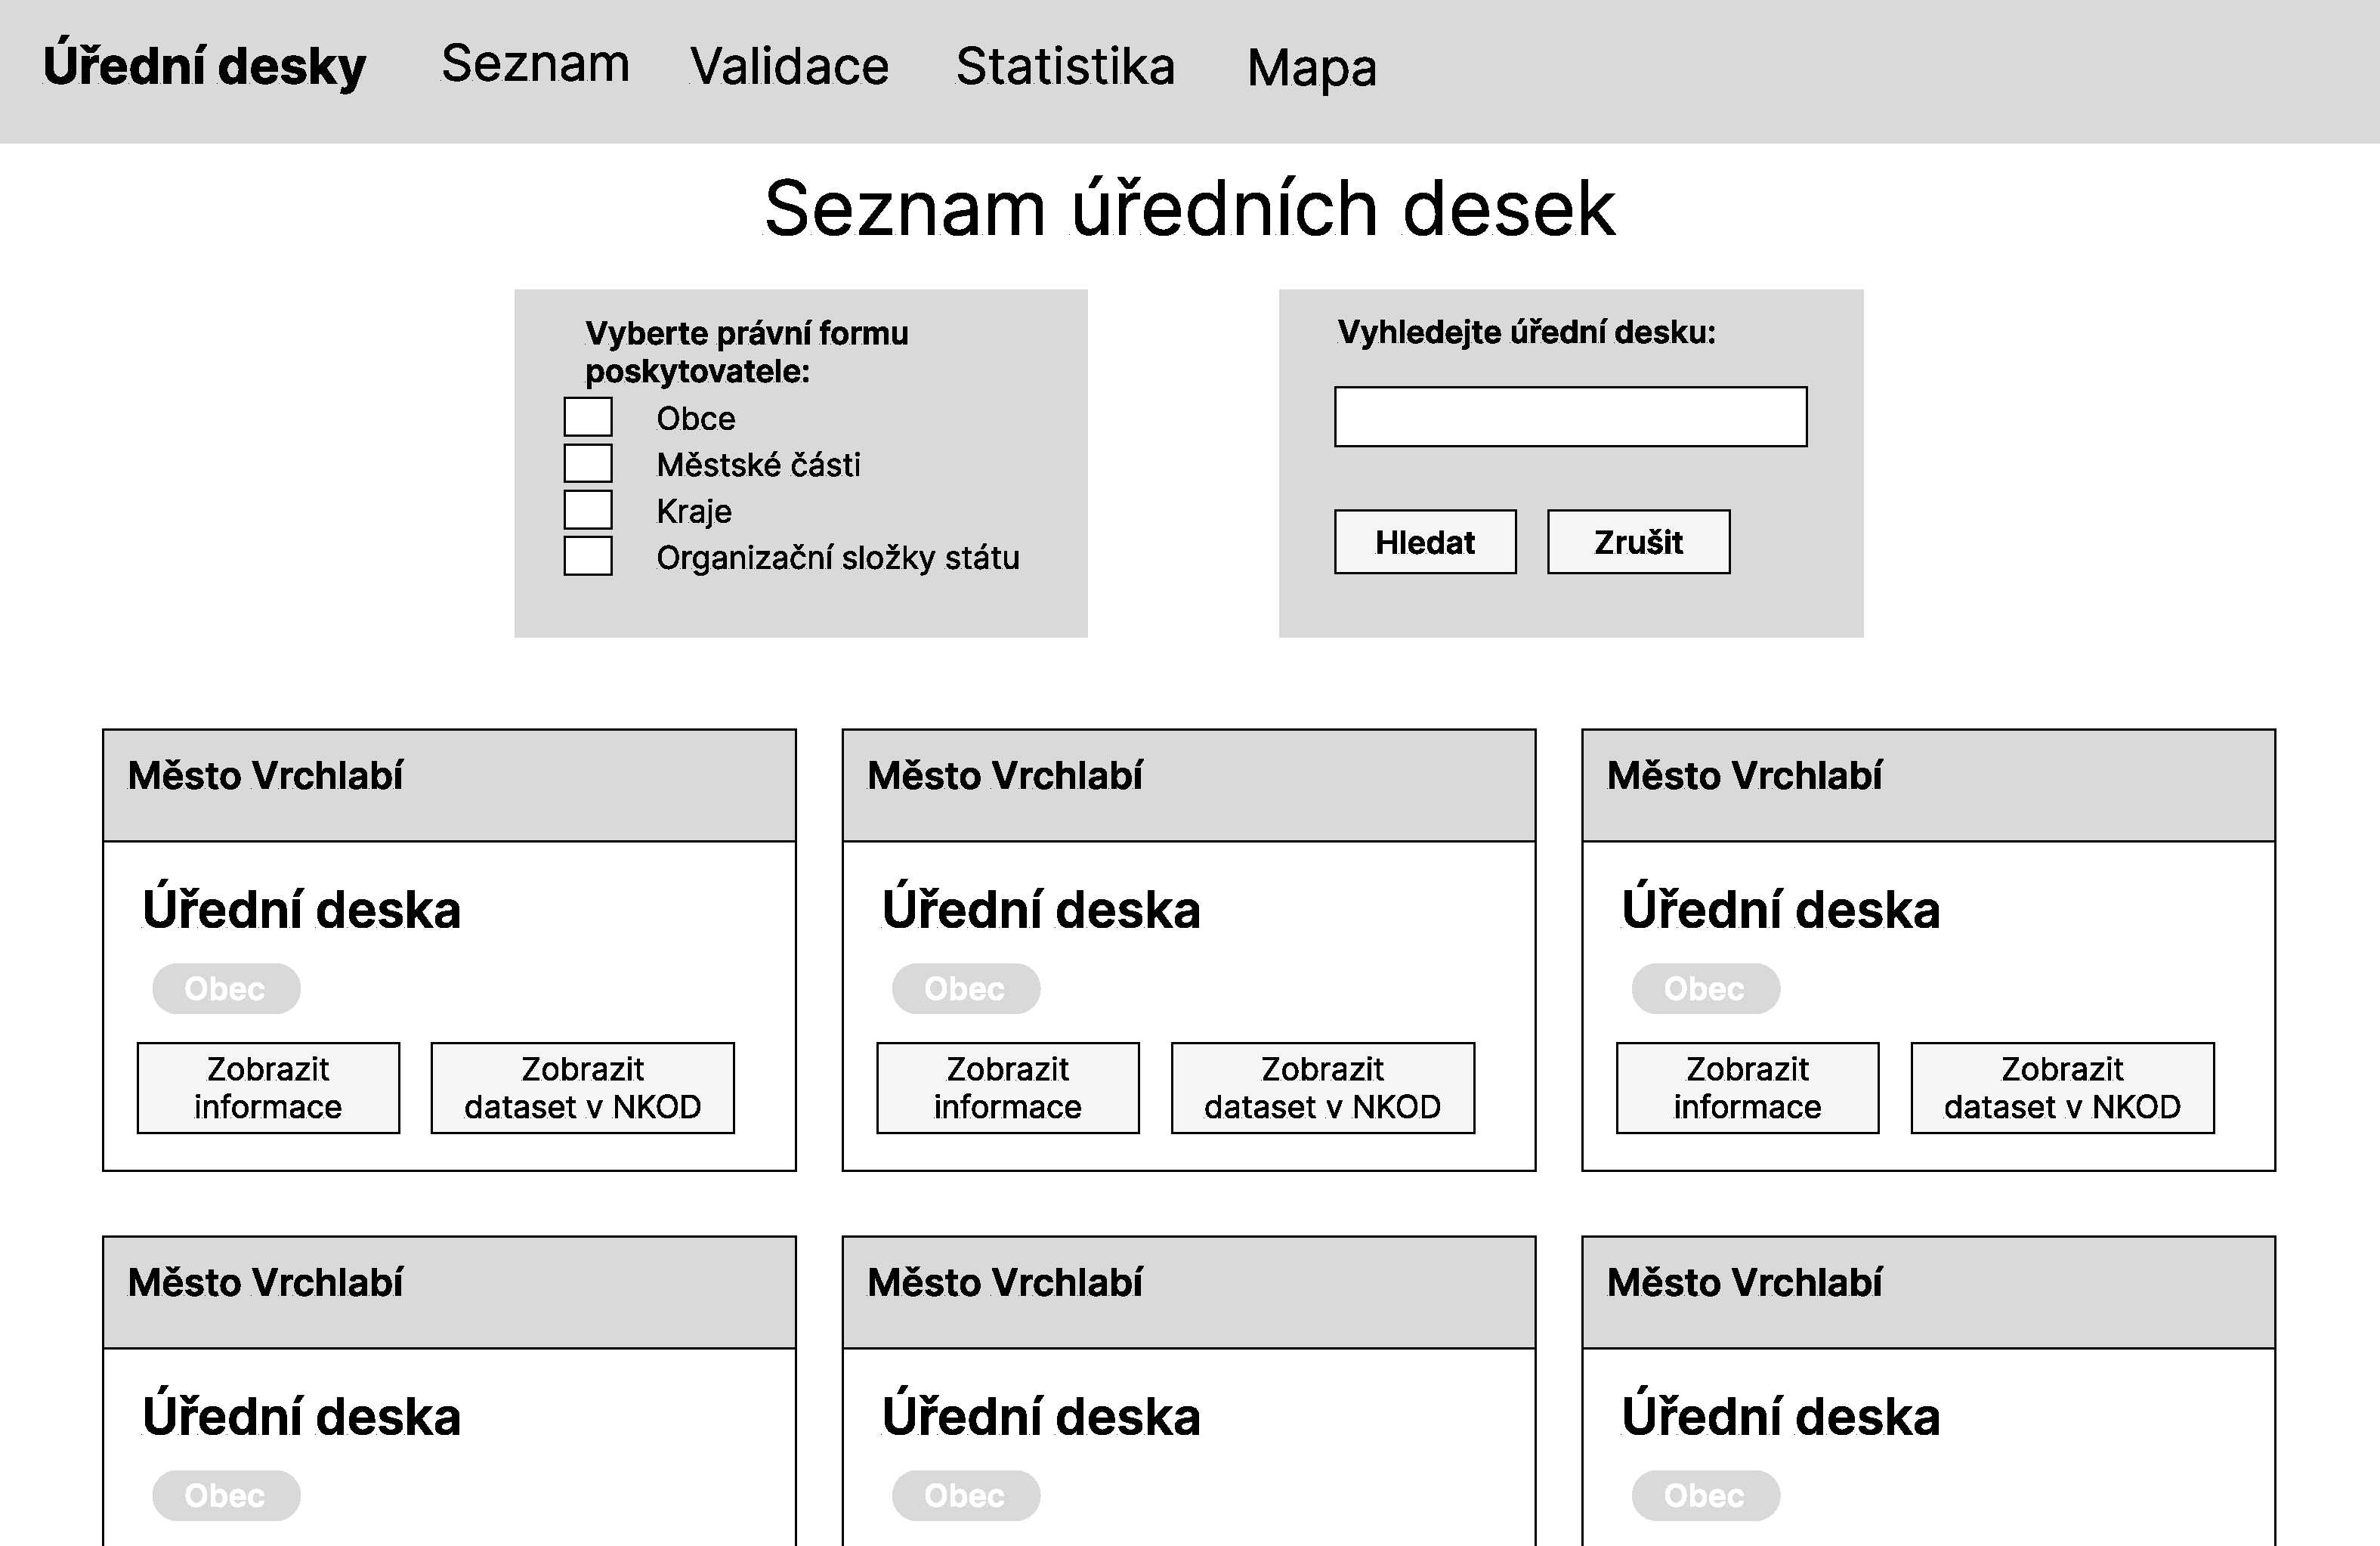
\includegraphics[width=1\textwidth, frame]{cs/obrazky/wireframes/wireframe_seznam.pdf}
\caption{Návrh uživatelského rozhraní - Seznam úředních desek}
\label{fig:seznam}
\end{figure}

Podle požadavku \textbf{V01} aplikace bude zobrazovat seznam všech úředních desek zveřejněných v NKOD podle OFN pro úřední desky. Pro reprezentaci úřední desky v seznamu je možné použít metadata, která získáme z NKOD při získání datové sady úřední desky, tedy název desky a název poskytovatele. Používáme pouze tato data, abychom mohli zobrazit seznam úředních desek bez nutnosti stahovat distribuce všech desek.

V seznamu bude možné vyhledat úřední desku podle názvu poskytovatele nebo názvu desky (požadavek \textbf{V02}). Bude k tomu sloužit formulář pro hledání. 

Modul dále umožní filtrování úředních desek podle právní formy poskytovatele (požadavek \textbf{V03}). Při analýze dat jsme objevili 4 hlavní právní formy poskytovatelů dat:
\begin{itemize}
    \item obce
    \item městské části a městské obvody
    \item kraje
    \item organizační složky státu
\end{itemize}
Pro tyto kategorie bude aplikace podporovat filtrování desek. Organizace jiných právních forem buď svoje úřední desky neposkytují, nebo se jedná o nižší jednotky desek, proto jsme pro ně vytvořili souhrnnou kategorii ostatní. Do této kategorie spadá i několik úředních desek poskytovatelů, kteří v RPP nemají uvedenou svoji právní formu, aplikace ji tedy nemůže zjistit.

Úřední desky v seznamu budou pro odlišení toho, do které spadají kategorie, obsahovat označení právní formy poskytovatele. Dále budou obsahovat odkaz na datovou sadu dané úřední desky v NKOD, jako možnost prohlédnout si syrová data z úřední desky, a také odkaz na vizualizaci informací na dané úřední desce (požadavek \textbf{V04}).

Na obrázku \ref{fig:seznam} najdeme návrh uživatelského rozhraní pro seznam úředních desek. V horní části obrazovky je umístěný navigační panel, pomocí kterého je možné přepínat mezi jednotlivými částmi aplikace. Dále na stránce najdeme dva formuláře, levý slouží pro filtrování a pravý pro vyhledávání úředních desek. Pod formuláři následuje seznam úředních desek, kde každá deska je reprezentovaná jednou kartičkou.



Seznam úředních desek je stránkovaný. Při načtení se zobrazí pouze prvních 20 desek. Ostatní desky je možné zobrazit zmáčknutím tlačítka \textit{Zobrazit další}, což přidá dalších 20 desek, nebo je možné načíst všechny desky zmáčknutím tlačítka \textit{Zobrazit vše}. Tato tlačítka jsou umístěná ve spodní části stránky, jejich návrh můžeme vidět na obrázku \ref{fig:paging}.

\begin{figure} 
\begin{center}
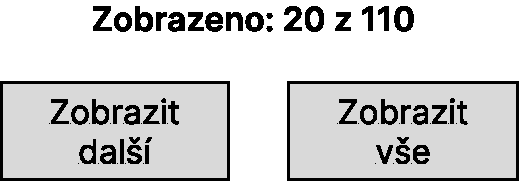
\includegraphics[width=0.3\textwidth]{cs/obrazky/wireframes/wireframe_paging.pdf} 
\end{center}
\caption{Návrh uživatelského rozhraní - Stránkování}
\label{fig:paging}
\end{figure}

\subsubsection{Detail úřední desky}

V detailu úřední desky bude možné si prohlédnout informace zveřejněné na této úřední desce (požadavek \textbf{V04}). Pro detail úřední desky použijeme data z distribuce datové sady, tedy metadata desky a informací, která odpovídají OFN pro úřední desky. Detail úřední desky bude obsahovat:
\begin{itemize}
    \item název desky
    \item název poskytovatele dat v NKOD
    \item název provozovatele desky, který je uveden v distribuci
    \item seznam všech informací na úřední desce setříděný podle data vyvěšení (požadavek \textbf{V05})
\end{itemize}

Každá informace v detailu desky bude mít následující položky (pokud jsou tyto položky přítomné v distribuci desky): 
\begin{itemize}
    \item název informace
    \item datum vyvěšení
    \item datum, do kterého je informace relevantní
    \item odkaz na obsah informace na elektronické stránce dané úřední desky
    \item přílohy (pokud má)
\end{itemize}

V informacích bude možné vyhledávat pomocí formuláře obdobného jako při vyhledávání úředních desek v seznamu. Hledání budeme provádět na základě názvu informace (požadavek \textbf{P06})

Podle požadavku \textbf{P01} bude možné k detailu konkrétní desky přistoupit pomocí IRI datové sady, umístěním IRI do query parametru \uv{iri} v URL aplikace.

\begin{figure} 
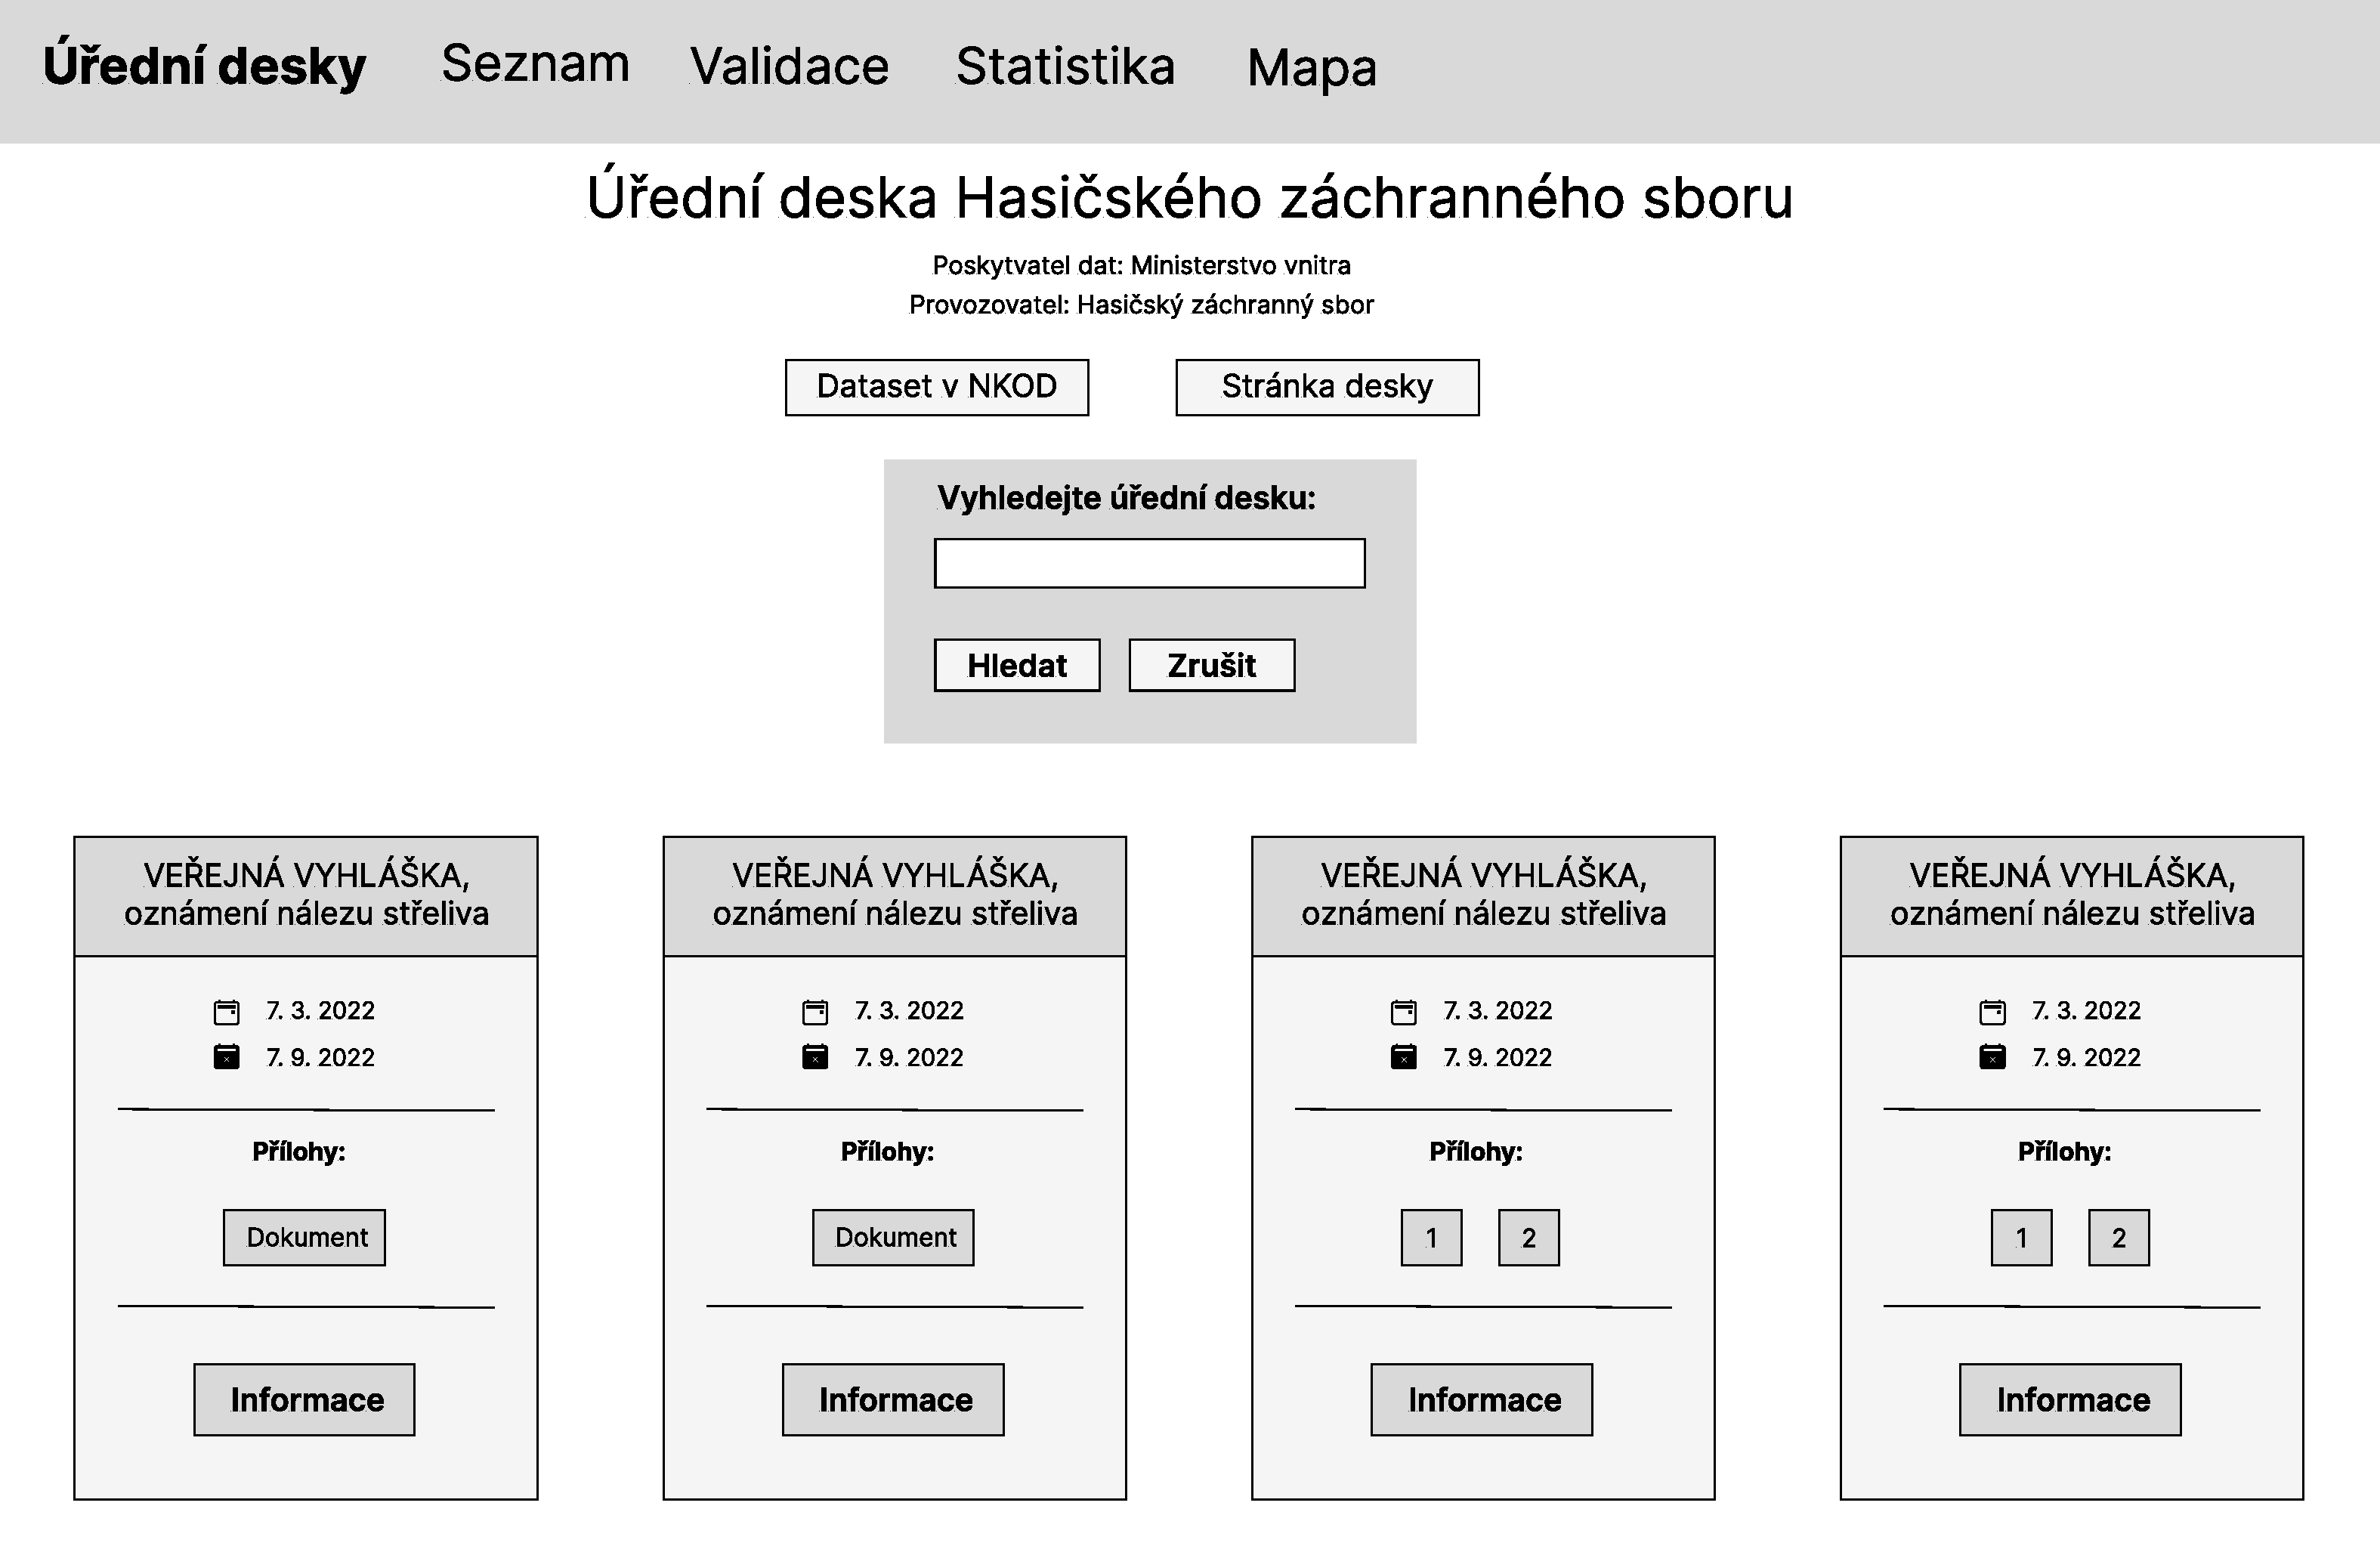
\includegraphics[width=\textwidth, frame]{cs/obrazky/wireframes/wireframe_detail.pdf}
\caption{Návrh uživatelského rozhraní - Detail úřední desky}
\label{fig:detail}
\end{figure}

\begin{figure} 
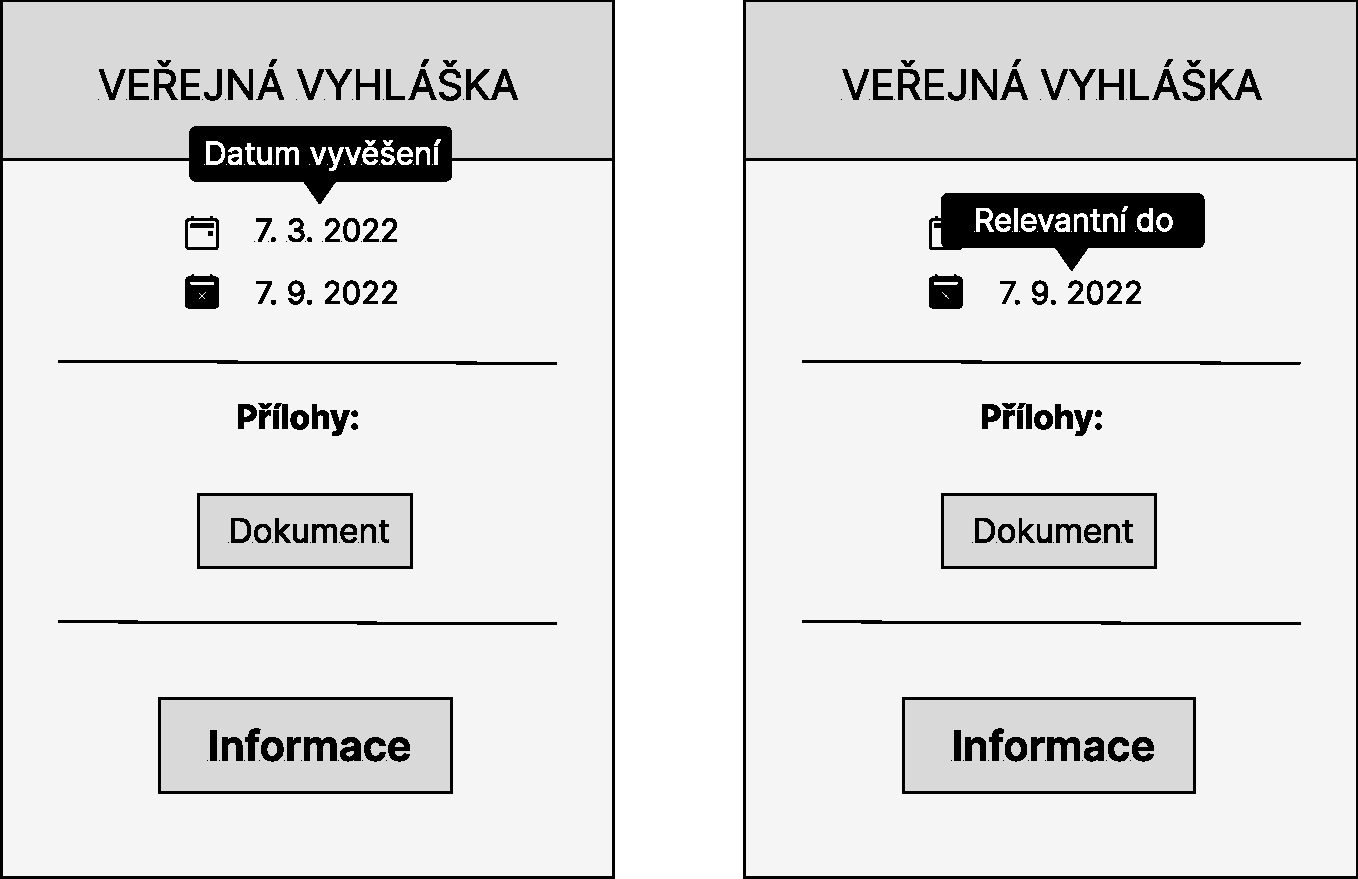
\includegraphics[width=1\textwidth]{cs/obrazky/wireframes/wireframe_detail_datum.pdf}
\caption{Návrh uživatelského rozhraní - Data platnosti informace - popisky}
\label{fig:detail-datum}
\end{figure}

Na obrázku \ref{fig:detail} vidíme návrh uživatelského rozhraní pro detail úřední desky. Na obrázku najdeme formulář pro vyhledání úřední desky a kartičky, které představují jednotlivé informace. Na kartičkách si všimneme dvou způsobů, kterými jsou zobrazeny přílohy informace. Pokud má informace pouze jednu přílohu, zobrazíme ji jako tlačítko s nápisem \textit{Dokument} (první dvě informace), pokud má příloh více, zobrazíme je jako očíslovaná tlačítka (druhé dvě informace). Tlačítko \textit{Informace} vede na URL, na kterém je informace zveřejněná.

V horní části kartičky s informací jsou dvě data --- datum vyvěšení a datum skončení relevance. Pro jejich znázornění jsme zvolili ikony, aby se textové popisky dat na kartičkách příliš neopakovaly. Pro větší přehlednost se při najetí myší na datum zobrazí jeho popisek, jak je vidět na obrázku \ref{fig:detail-datum}



Informace v detailu desky jsou stránkované stejným způsobem, jako kartičky s deskami v seznamu úředních desek.

\subsubsection{Mapa úředních desek}

\begin{figure} 
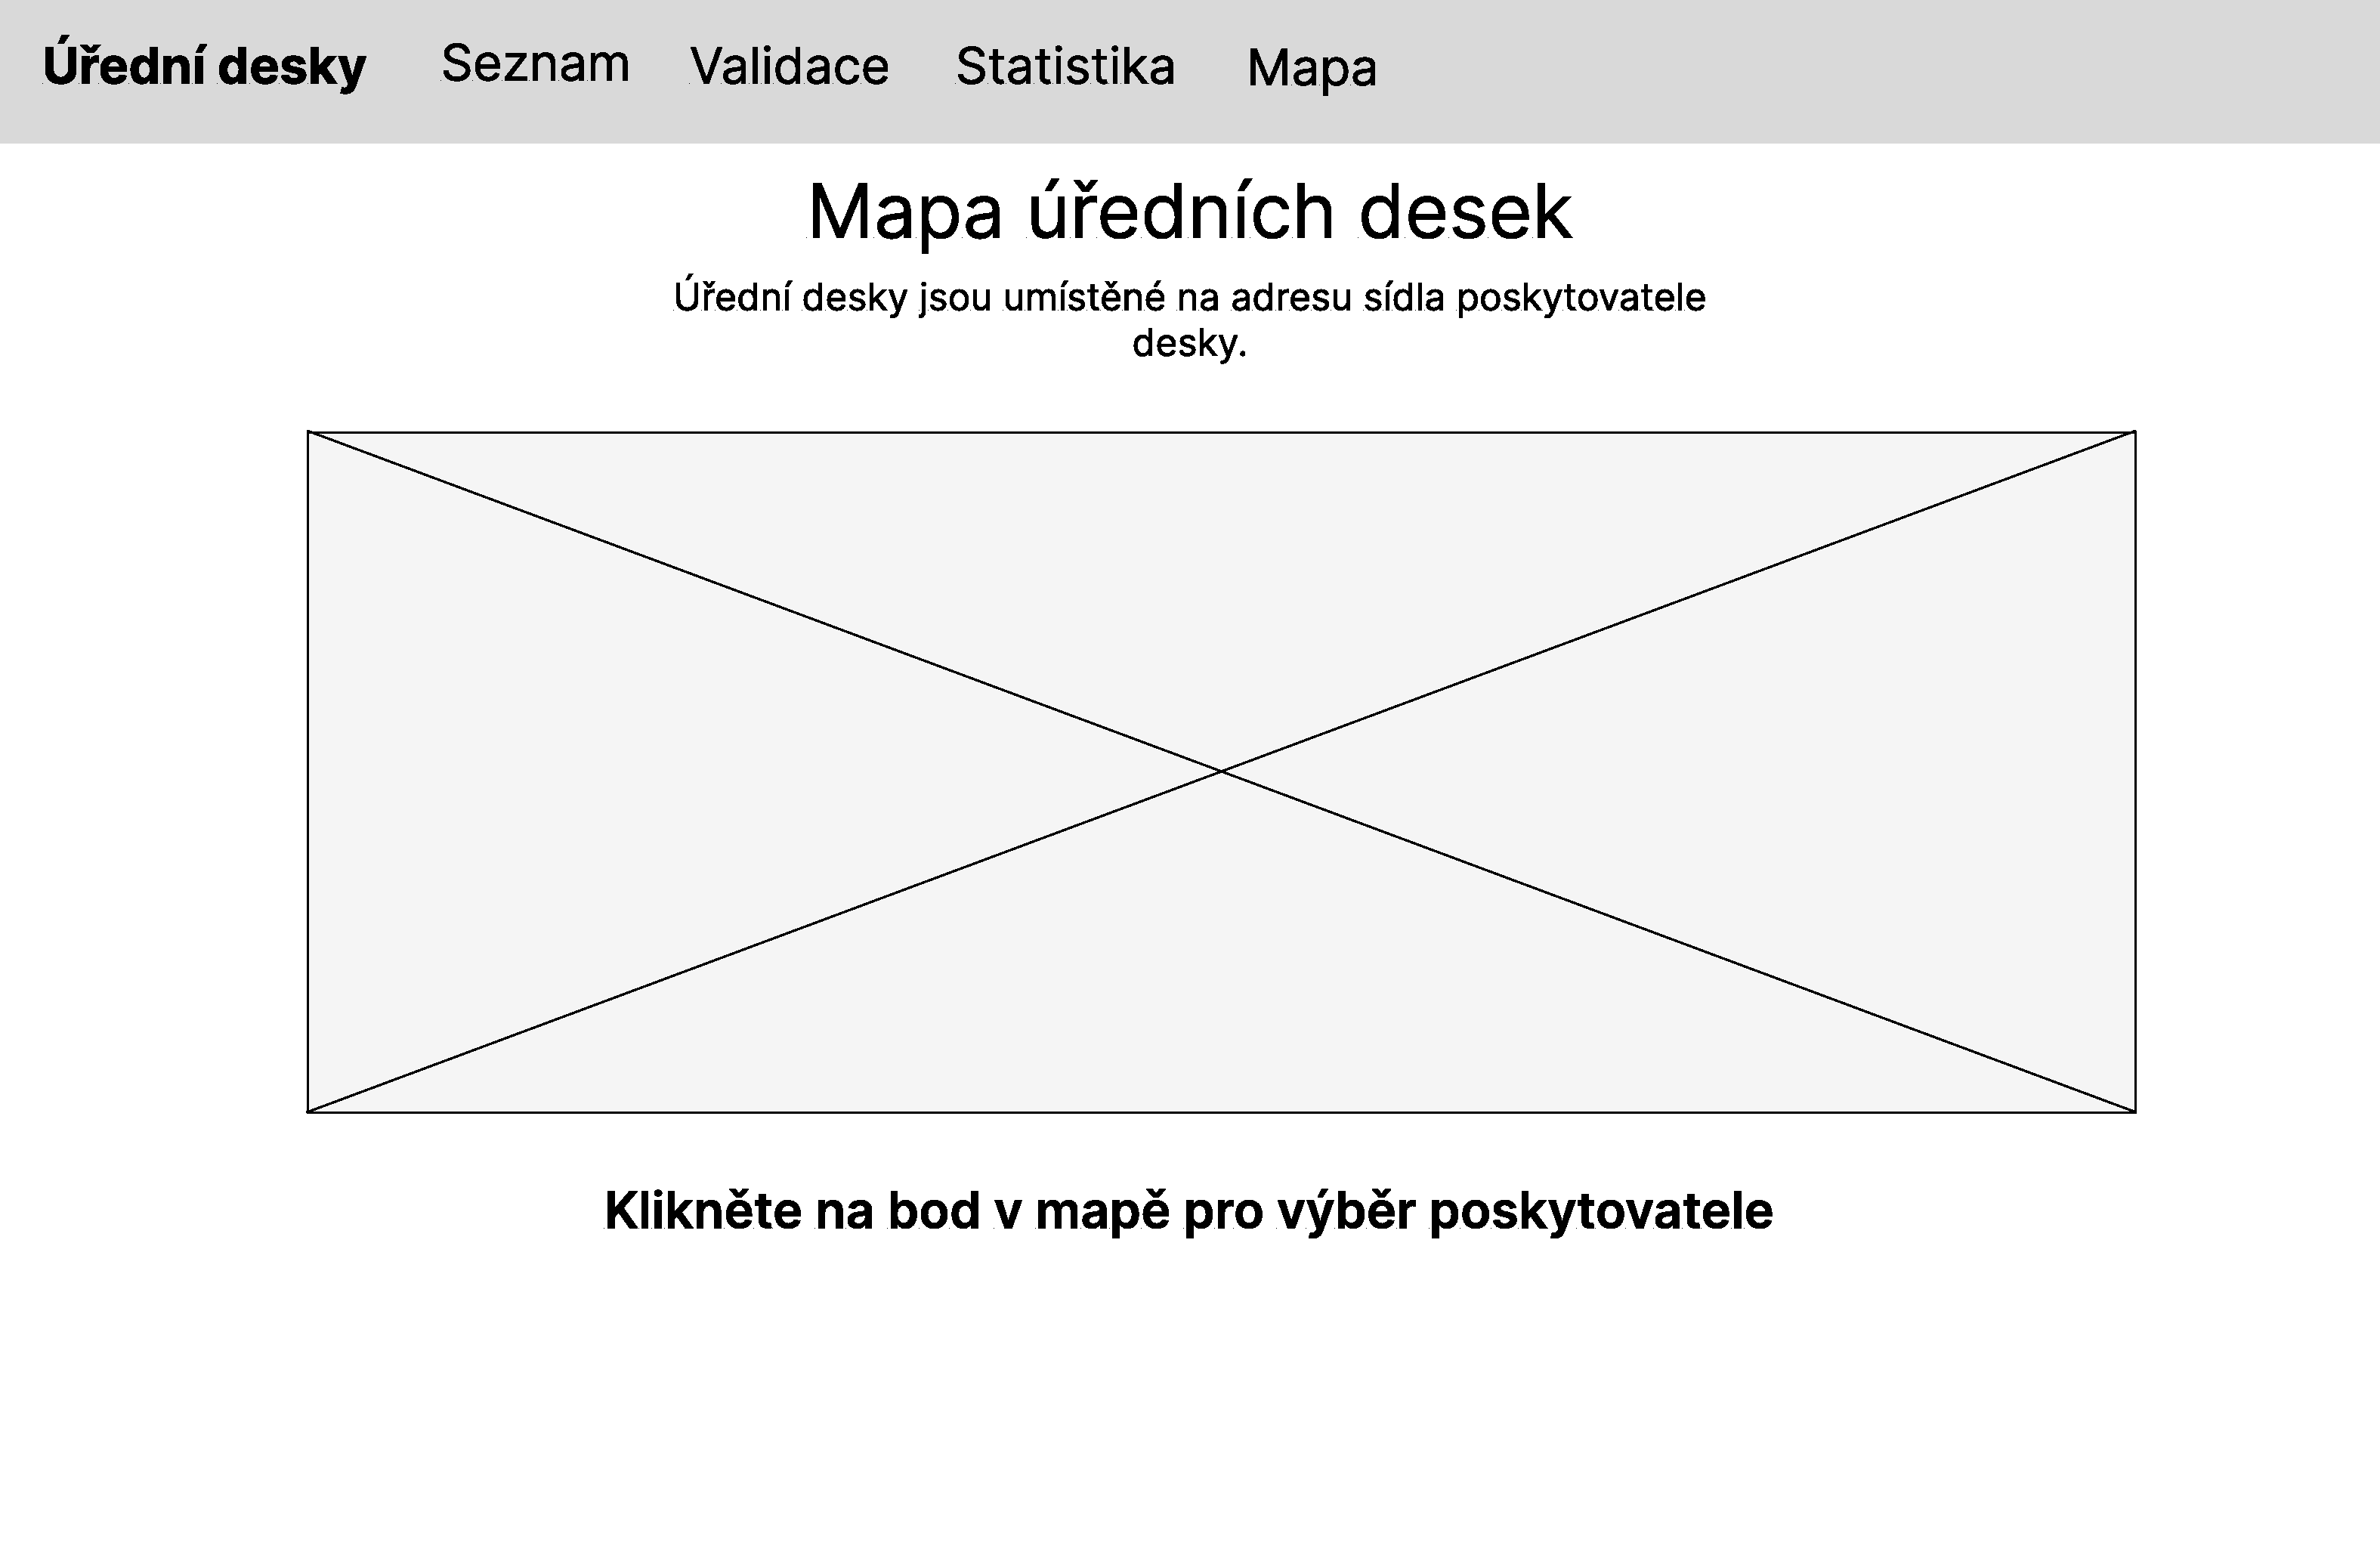
\includegraphics[width=\textwidth, frame]{cs/obrazky/wireframes/wireframe_mapa.pdf}
\caption{Návrh uživatelského rozhraní - Mapa úředních desek}
\label{fig:mapa}
\end{figure}

Kromě vizualizace úředních desek v podobě seznamu bude modul také nabízet vizualizaci na mapě (požadavek \textbf{V07}). Mapa bude po načtení přiblížená tak, aby ukazovala mapu ČR. Na mapě budou zobrazené body, reprezentující poskytovatele úředních desek. Body budou umístěné na souřadnice adresy sídla poskytovatele získané z RPP. Při kliknutí na bod v mapě se zobrazí všechny úřední desky, které daný poskytovatel zveřejňuje. Body budou barevně odlišené podle právní formy poskytovatele.

Na obrázku \ref{fig:mapa} vidíme návrh uživatelského rozhraní mapy úředních desek.


\subsection{Validace}

Modul Validace obsahuje všechny funkcionality, které se týkají validace dat z úředních desek. Cílem validace je ověřit, že distribuce dané úřední desky obsahuje všechny doporučené atributy podle specifikace OFN (požadavky \textbf{P02} a \textbf{P03}). V případě, že distribuci úřední desky nelze stáhnout, aplikace na to uživatele upozorní a nabídne možná řešení.

Nabízená řešení vychází z analýzy příčin způsobujících chyby při stahování. Objevili jsme následující příčiny (příčiny jsou seřazené od nejčastějších):
\begin{enumerate}
    \item Špatné nastavení hlavičky \uv{Access-Control-Allow-Origin}, kdy je distribuce desky správně zveřejněná, ale není možné ji stáhnout strojově požadavkem z kódu.
    \item URL distribuce uvedené v NKOD je neplatné, nebo nevede na soubor s distribucí.
    \item Neplatný SSL certifikát stránky.
\end{enumerate}
Aplikace tedy uživatele upozorní na uvedené 3 příčiny a nabídne odkazy na další informace.

Strukturou je modul Validace podobný modulu Vizualizace. Obsahuje seznam stručných výsledků validací úředních desek a detail validace pro každou desku. Seznam je možné filtrovat podle typu poskytovatele a vyhledávat v něm (požadavky \textbf{P06} a \textbf{P07}).  V seznamu je pro každou desku zobrazeno stručné shrnutí validace:
\begin{itemize}
    \item je možné stáhnout distribuci (ano/ne)
    \item metadata celé desky obsahují všechny doporučené atributy (ano/ne)
    \item metadata všech informací na desce obsahují všechny doporučené atributy (ano/ne)
    \item celkový počet informací na desce
\end{itemize}
Ze shrnutí je možné otevřít detail validace desky.

Rozhodli jsme se, že seznam výsledků validace budeme zobrazovat v tabulce. Výsledky validace mají charakter tabulkových dat, kdy jsou pro každou úřední desku zobrazeny hodnoty v několika kategoriích, proto je zobrazení tabulkou pro tato data přirozenou a přehlednou volbou. 

Nevýhodou tabulky je její špatná přizpůsobivost užším obrazovkám, jako jsou mobilní zařízení. Nicméně jsme usoudili, že uživatel s rolí poskytovatel dat, bude nejspíše aplikaci používat v rámci pracovní doby na počítači, tedy je zde tabulka vhodná. Při otevření aplikace na úzkém displeji zobrazíme uživateli upozornění, že je lepší tento modul aplikace prohlížet na širším displeji.

Na obrázku \ref{fig:validace} vidíme návrh uživatelského rozhraní pro tabulku s přehledem validace. Řádky tabulky jsou barevně zvýrazněné podle výsledku validace dané úřední desky --- červeně, pokud nelze stáhnout distribuci a žlutě, pokud chybí některé doporučené atributy.

\begin{figure} 
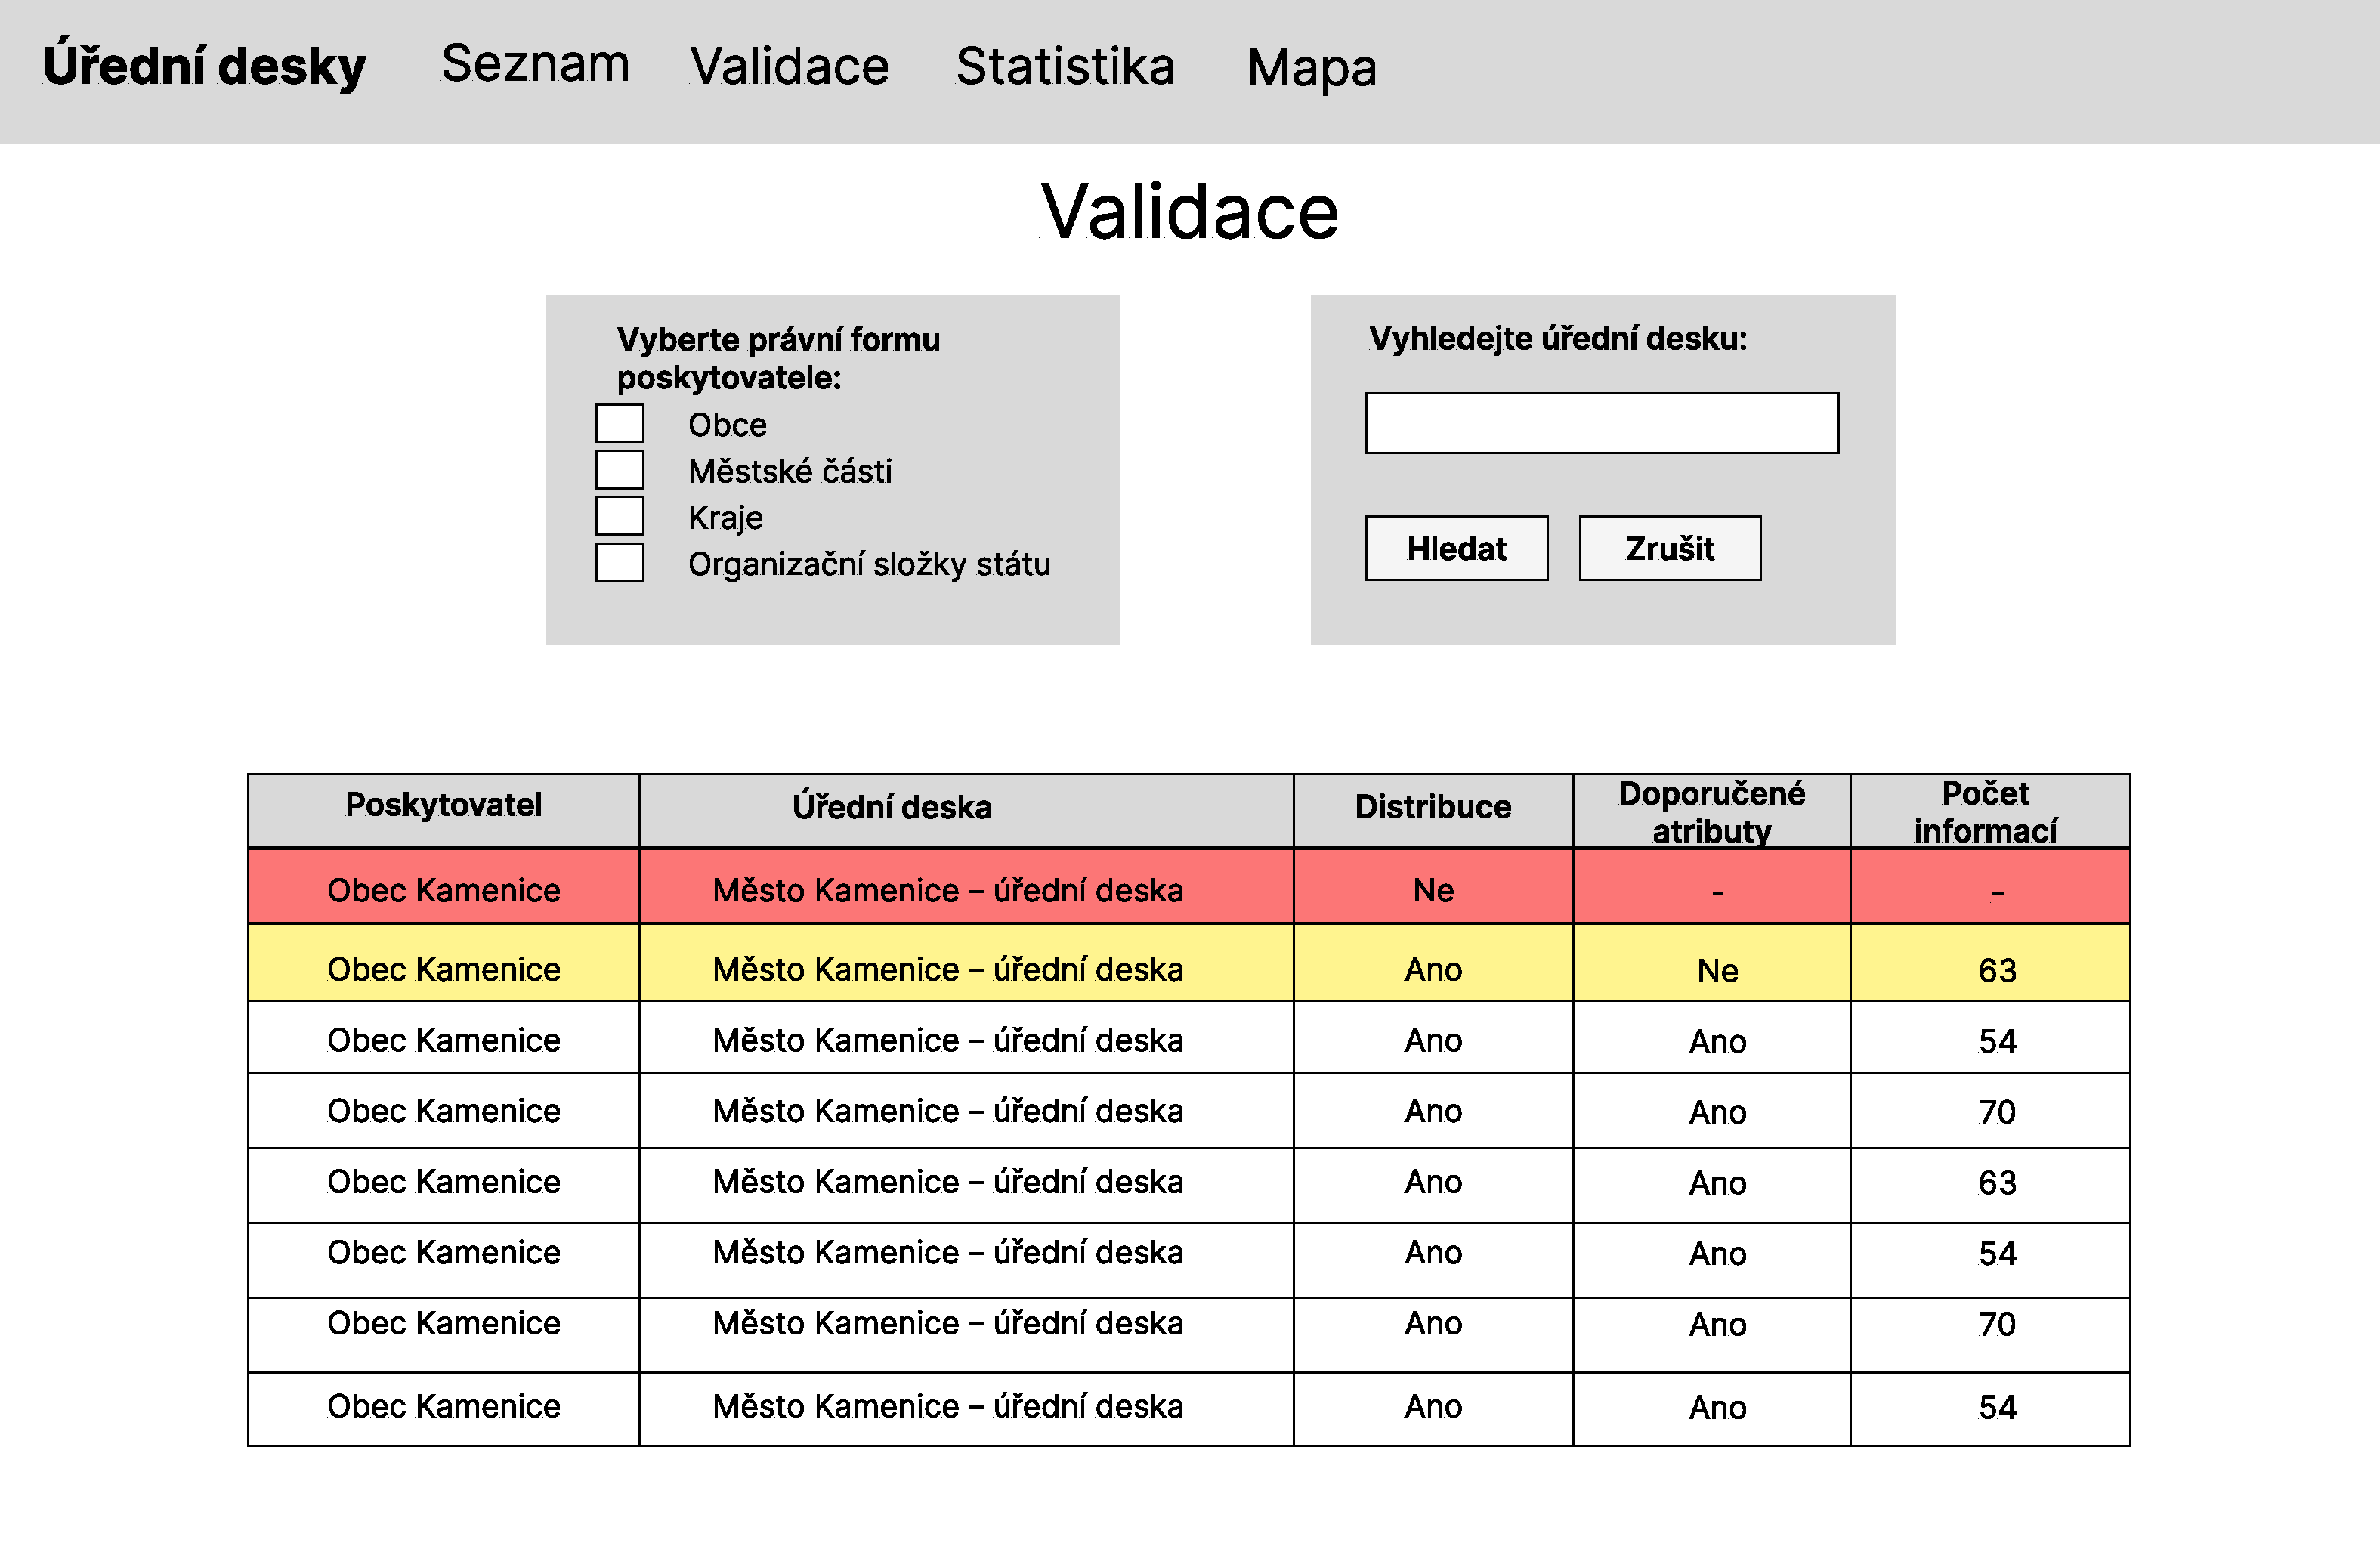
\includegraphics[width=\textwidth, frame]{cs/obrazky/wireframes/wireframe_validace.pdf}
\caption{Návrh uživatelského rozhraní - Přehled validace}
\label{fig:validace}
\end{figure}

Řádky tabulky s výsledky validace jsou stránkované stejným způsobem jako úřední desky v seznamu úředních desek.

\subsubsection{Detail validace úřední desky}

Na obrázku \ref{fig:validace-detail} je návrh uživatelského rozhraní pro detail validace úřední desky.

\begin{figure} 
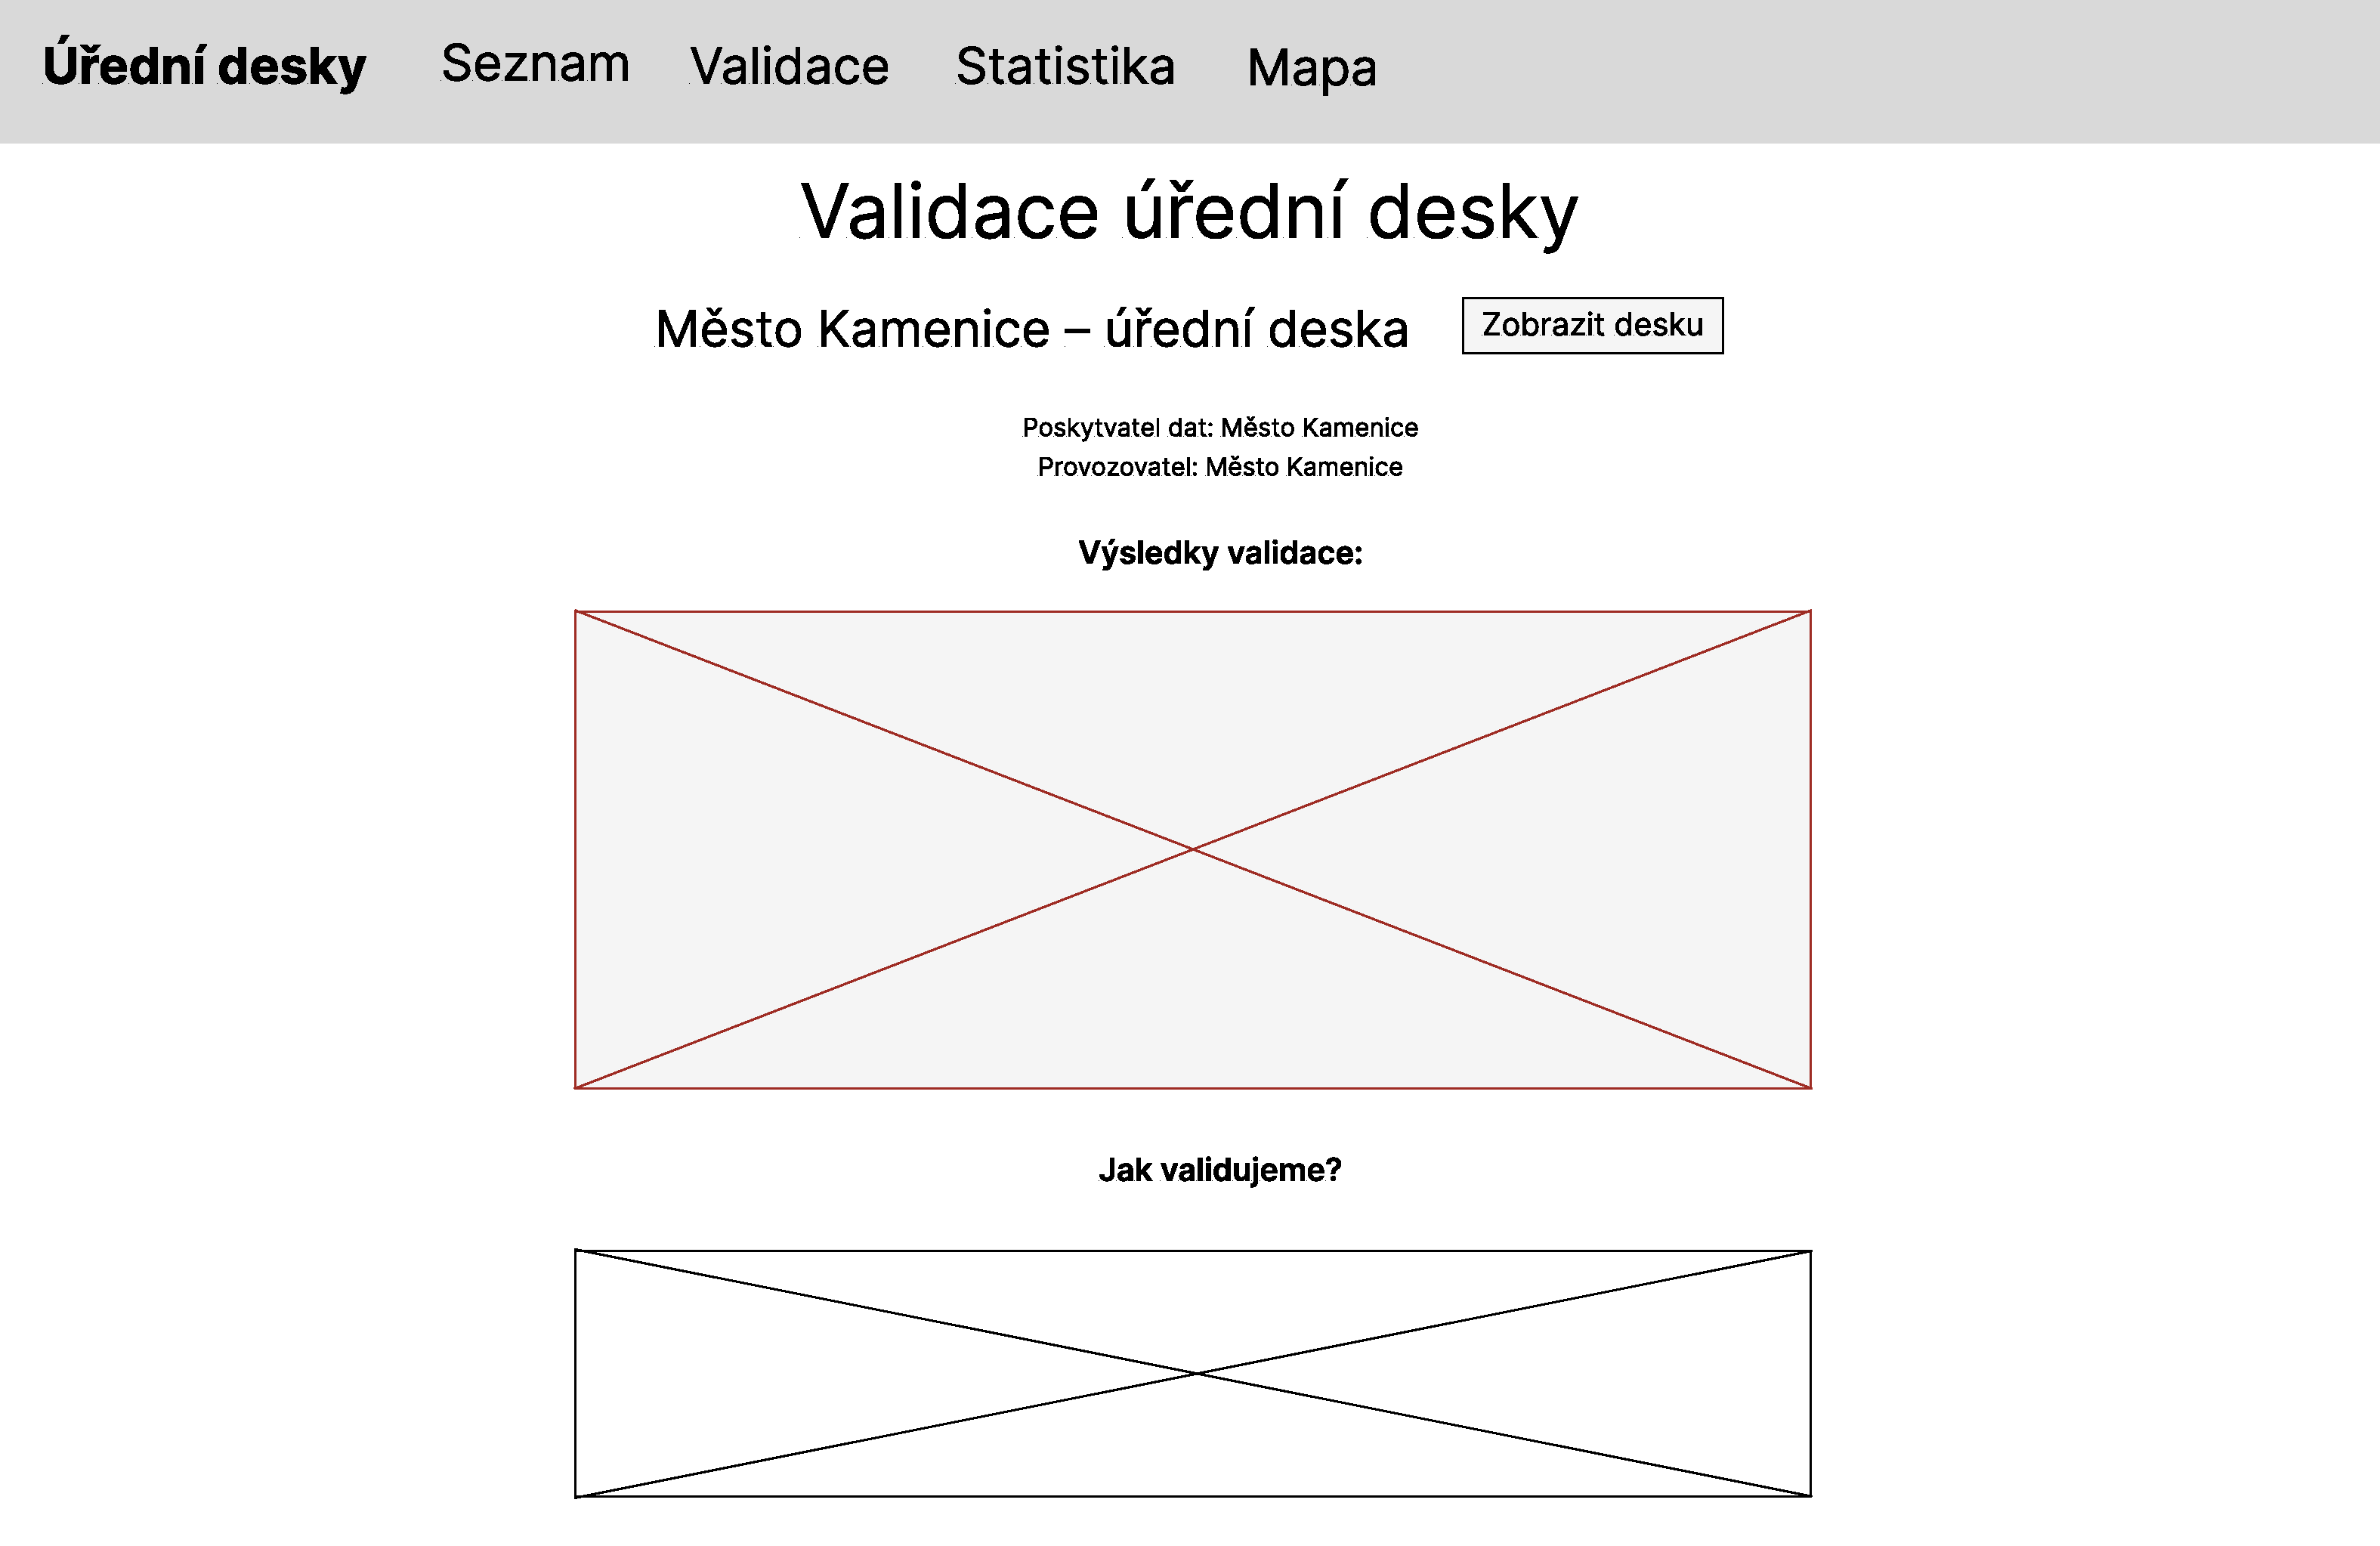
\includegraphics[width=\textwidth, frame]{cs/obrazky/wireframes/wireframe_validace_detail.pdf}
\caption{Návrh uživatelského rozhraní - Detail validace}
\label{fig:validace-detail}
\end{figure}

V horní části najdeme název úřední desky a odkaz na vizualizaci desky, a také informace o poskytovateli a provozovateli desky. Dále je na stránce umístěn rámeček s výsledkem validace, který je barevně označený podle výsledku.

Pro úřední desku, jejíž distribuci nelze stáhnout se v rámečku zobrazí upozornění, které obsahuje URL distribuce, chybová hláška získaná z nepovedeného dotazu na stažení distribuce a možná řešení problému popsaná výše. Rámeček má červenou barvu.

Pro úřední desku, kde chybí některé doporučené atributy, je rámeček žlutý. Je v něm vypsáno, které atributy chybí. V případě, že chybí doporučené atributy v metadatech informace, jsou zobrazeny všechny informace, kde chybí atributy a u každé informace je uvedeno, o které atributy se jedná. 

Pokud distribuce úřední desky nemá nedostatky, obsahuje rámeček jenom krátkou informaci o úspěšné validaci a je zelený.

Na obrázku \ref{fig:validace-detail} je ukázaný případ, kdy distribuci desky není možné stáhnout.

V každém případě detail validace kromě výsledku validace nabízí i vysvětlení, jak se validuje, kde jsou popsané jednotlivé doporučené atributy a jejich význam v datech. Toto vysvětlení je v návrhu na obrázku  \ref{fig:validace-detail} umístěné místo rámečku pod nadpisem \textit{Jak validujeme?}.


\subsection{Statistika}

Modul Statistika se věnuje zobrazení statistik z validace dat a statistik poskytovatelů podle požadavků \textbf{N01} a \textbf{N02}. 

\subsubsection{Statistika validace}

Část, která se týká validace dat, bude obsahovat souhrnný stav validace v textovém popisu a na koláčovém grafu. Statistika bude složená z následujících údajů:
\begin{itemize}
    \item Celkový počet úředních desek zveřejněných jako otevřená data.
    \item Počet distribucí desek, které nebylo možné stáhnout.
    \item Počty desek, které neobsahují všechny doporučené atributy, rozdělené podle toho, kterým chybí atributy celé desky a atributy jednotlivých informací.
    \item Celkový počet desek s nedostatky (nestažitelná distribuce, chybějící atributy).
\end{itemize}

Tato část bude také obsahovat seznam všech desek s nedostatky. Pro každou desku v seznamu bude možné otevřít detail její validace v modulu Validace.

Na obrázku \ref{fig:stat-validace} je zobrazen návrh uživatelského rozhraní pro statistiku validace.

\begin{figure} 
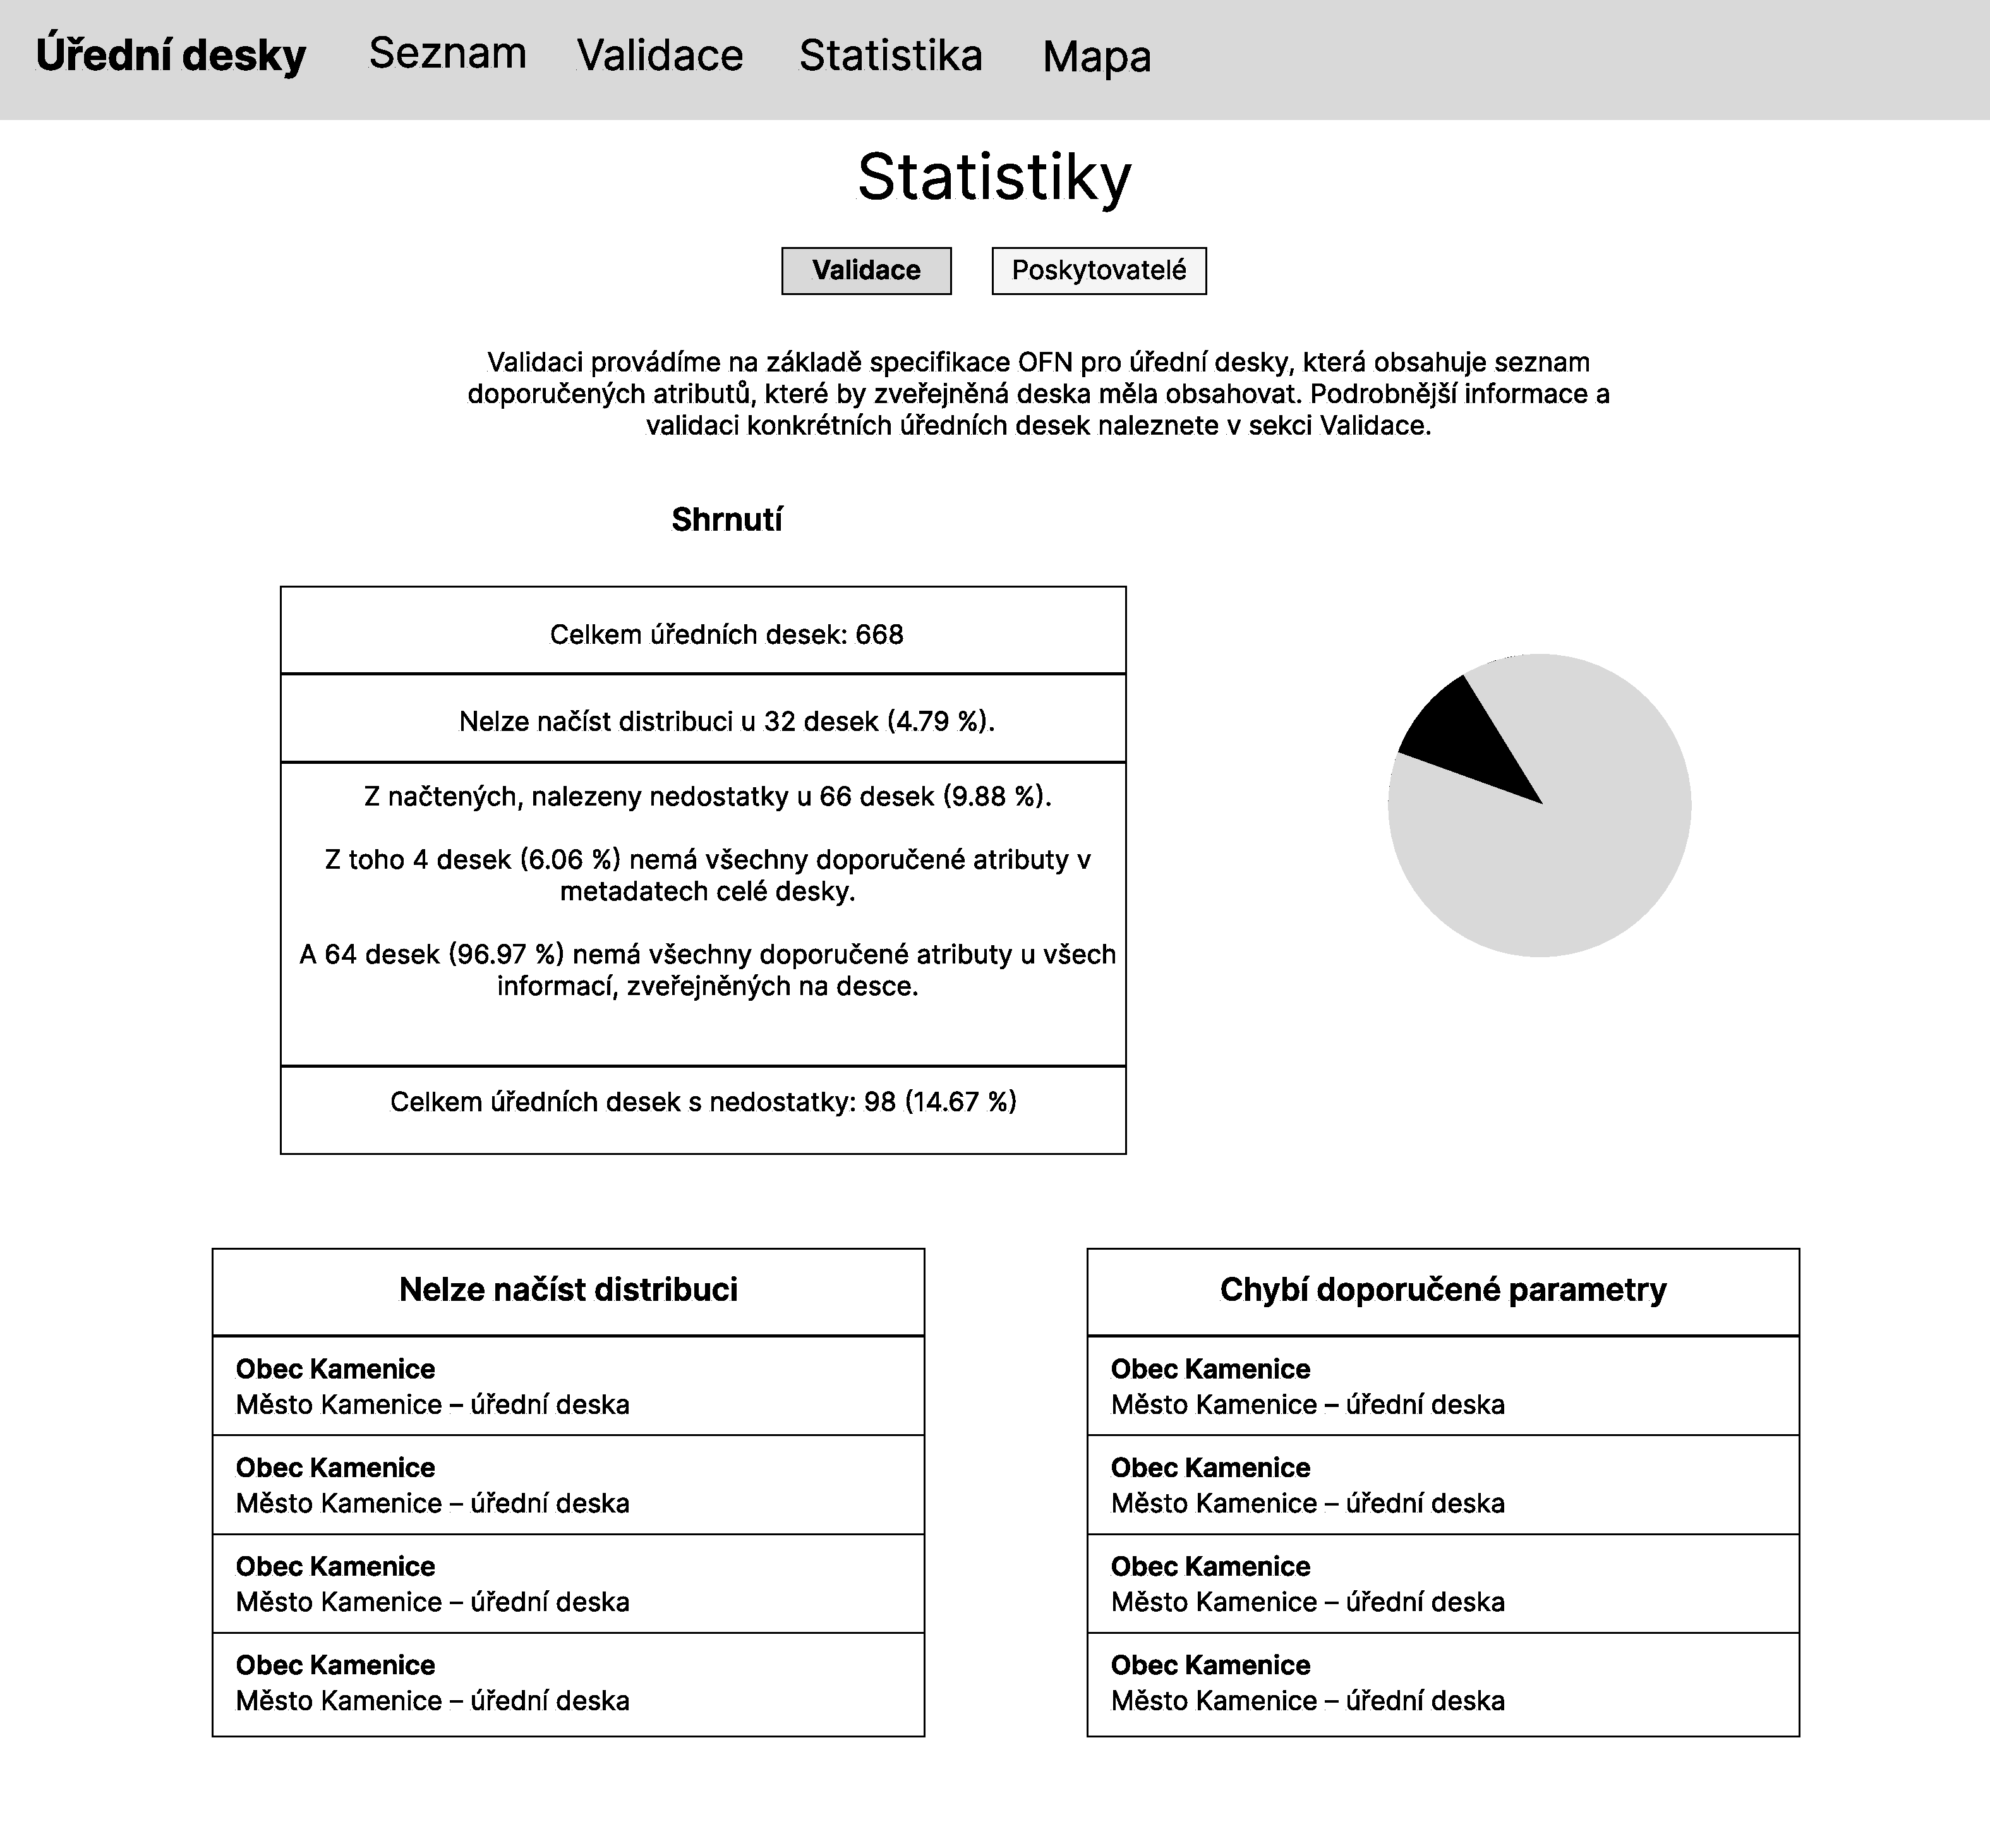
\includegraphics[width=\textwidth, frame]{cs/obrazky/wireframes/wireframe_statistika_validace.pdf}
\caption{Návrh uživatelského rozhraní - Statistika validace}
\label{fig:stat-validace}
\end{figure}

\subsubsection{Statistika poskytovatelů}

Druhá část modulu bude statistika poskytovatelů dat z úředních desek. Pro čtyři největší kategorie poskytovatelů --- obce, městské části a městské obvody, kraje a organizační složky státu --- bude na koláčových grafech zobrazeno, kolik ze všech orgánů dané právní formy poskytuje svoji úřední desku jako otevřená data.

Dále bude následovat seznam ostatních právních forem, s počtem existujících orgánů dané právní formy a z nich počet poskytovatelů úředních desek. Návrh uživatelského rozhraní pro tuto část můžeme vidět na obrázku \ref{fig:stat-poskyt}.

\begin{figure} 
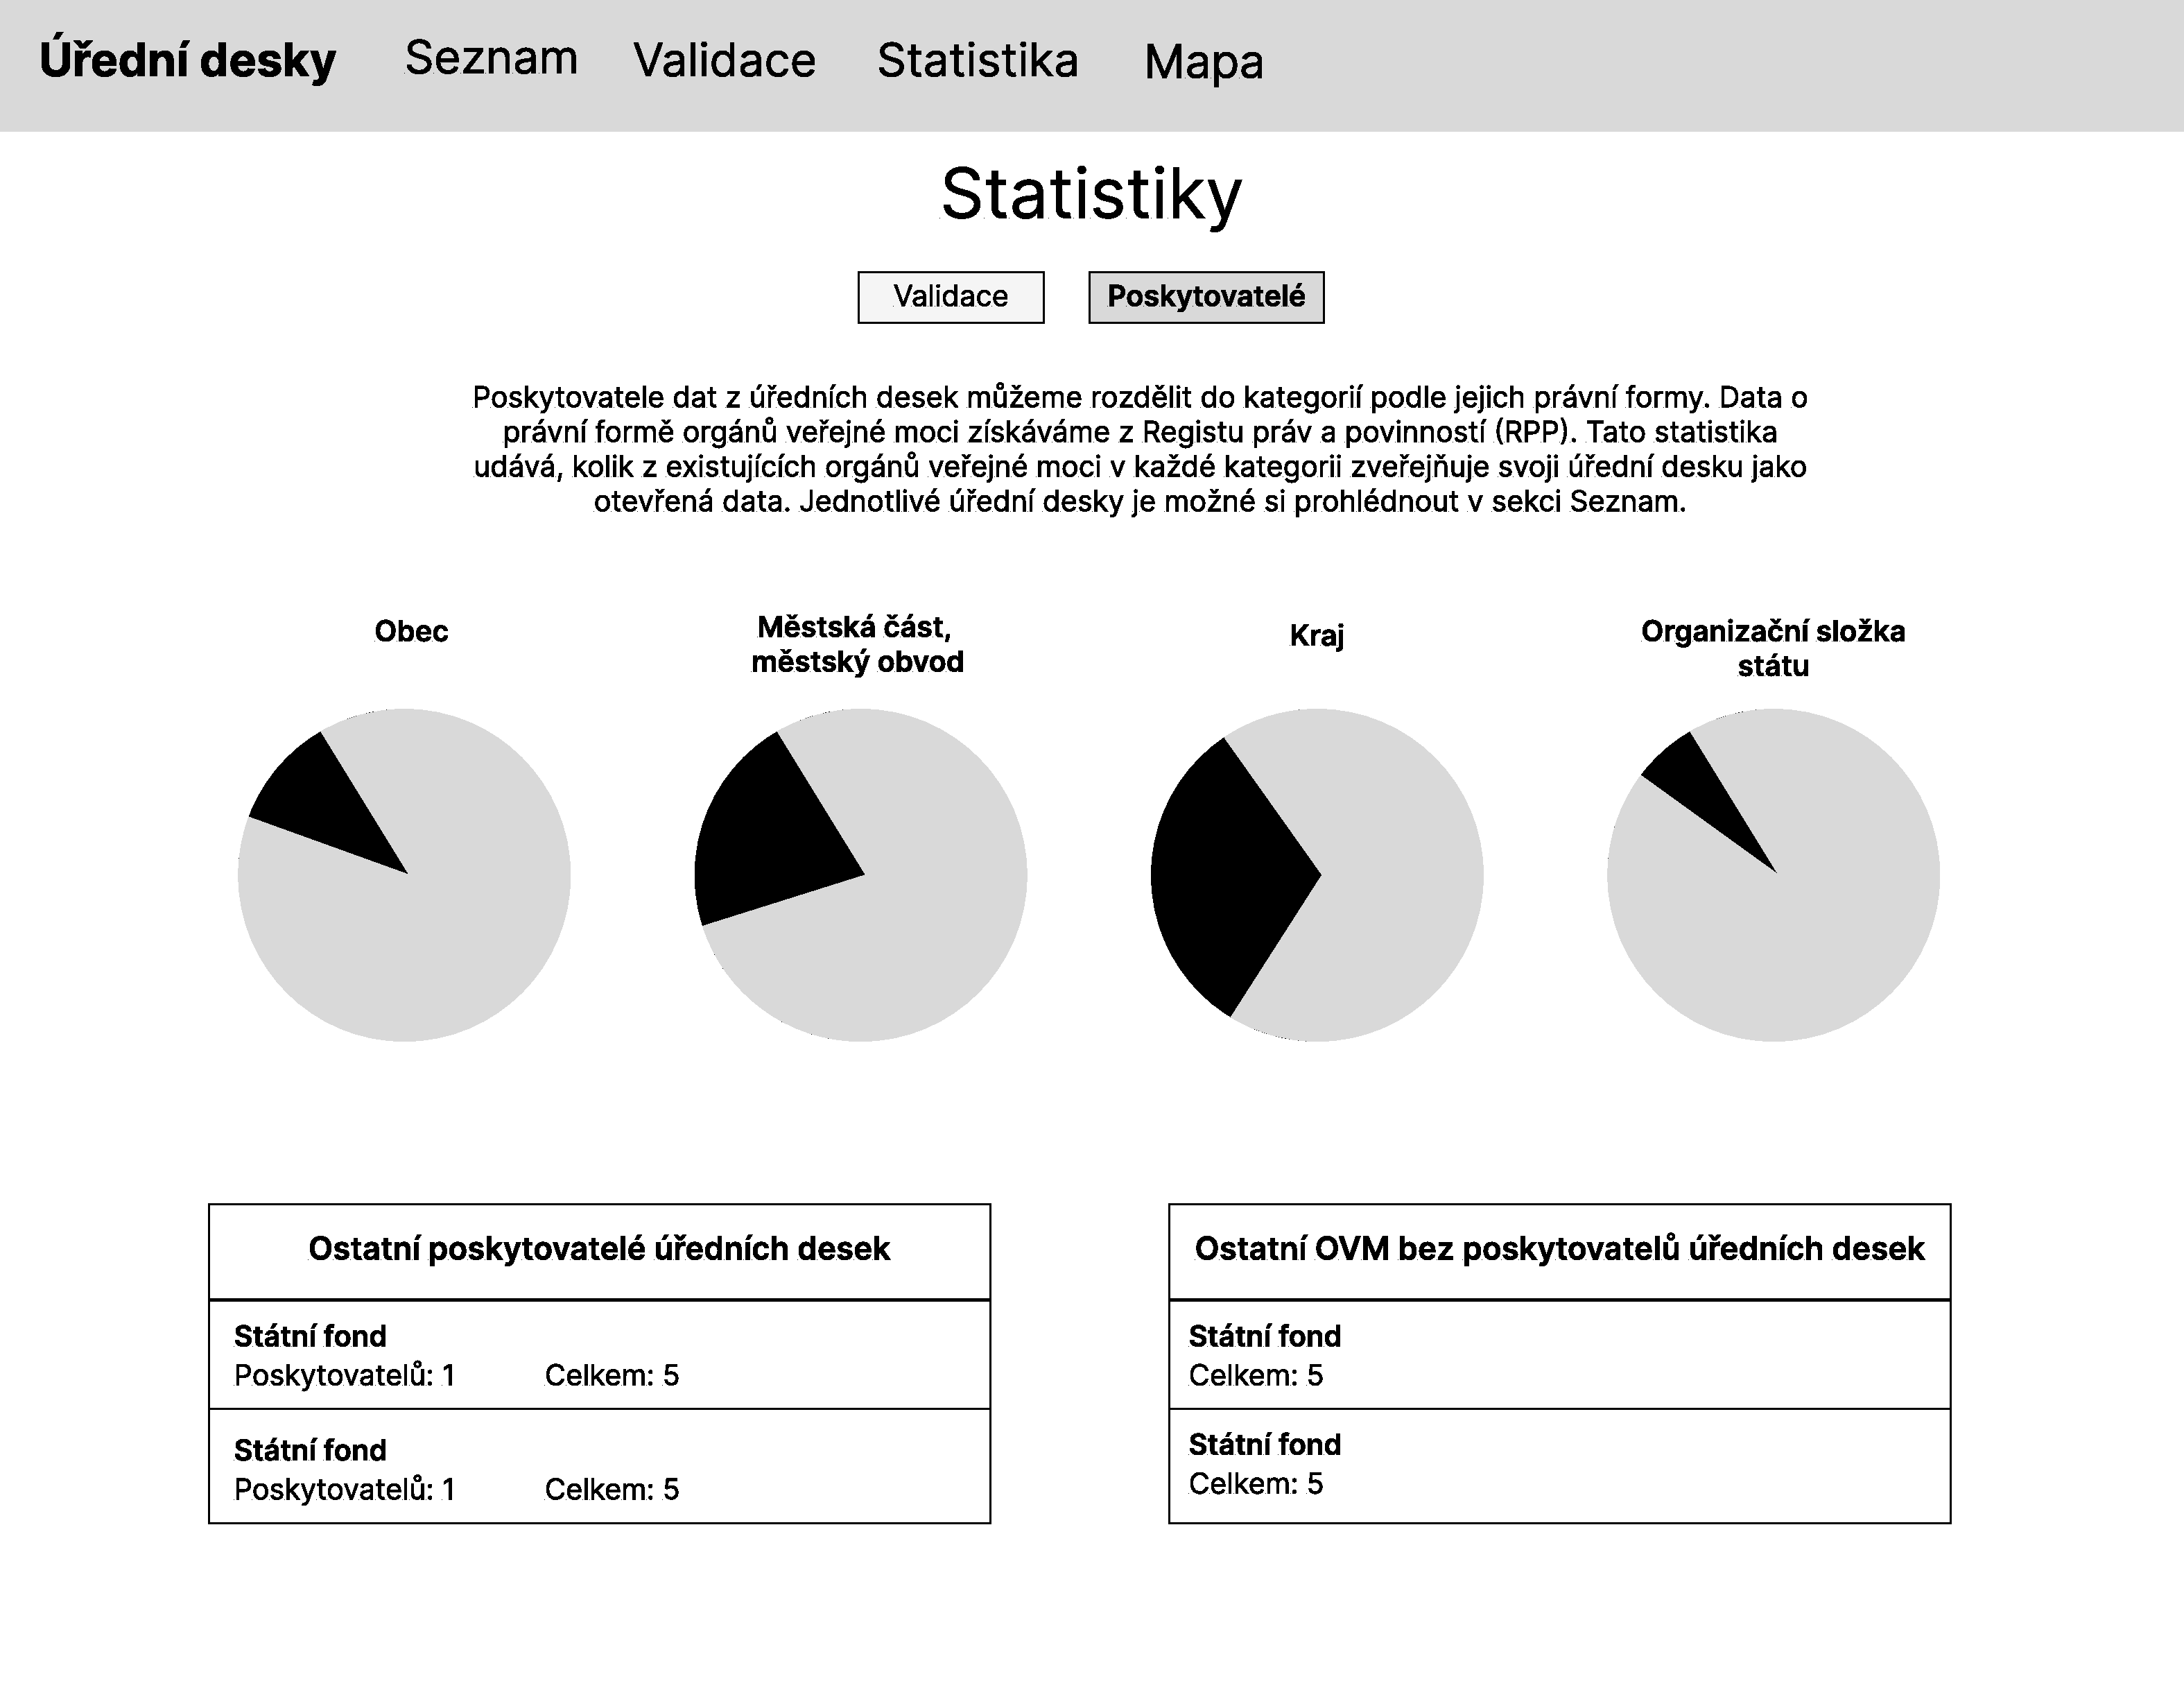
\includegraphics[width=\textwidth, frame]{cs/obrazky/wireframes/wireframe_statistika_poskytovatele.pdf}
\caption{Návrh uživatelského rozhraní - Statistika poskytovatelů}
\label{fig:stat-poskyt}
\end{figure}


\section{Architektura}\label{sec:architektura}

Aplikace je navržená jako \emph{single-page application} implementovaná na straně klienta. To znamená, že aplikace pracuje bez serveru pouze na straně klienta a obsah aplikace je dynamicky renderovaný na základě interakce s uživatelem.

Toto řešení jsme zvolili pro splnění požadavku \textbf{T01} (viz \autoref{sub:tech-poz}), podle kterého by mělo být nasazení aplikace zprostředkováno pomocí služby GitHub Pages \footnote{\url{https://docs.github.com/en/pages/getting-started-with-github-pages}}. Tato služba umožňuje beplatné hostování webových aplikací z repozitáře na GitHub\footnote{\url{https://github.com/}}. V rámci služby je možné hostovat pouze statický obsah, nebo obsah renderovaný na straně klienta.

Detaily sestavení a nasazení aplikace jsou popsané v kapitole Implementace (\autoref{kap:implementace}).


\begin{figure} 
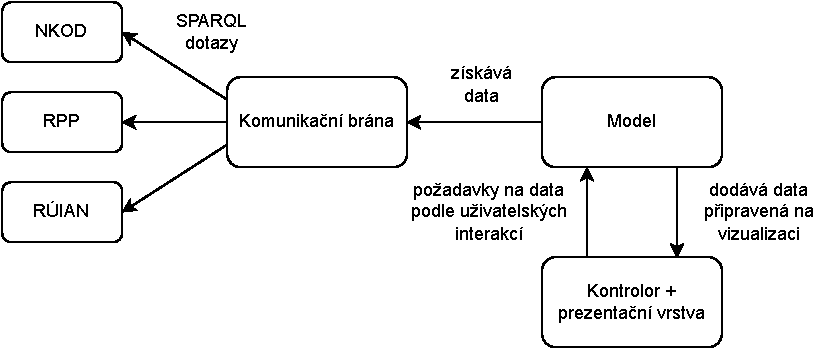
\includegraphics[width=\textwidth]{cs/obrazky/architektura_diagram.pdf}
\caption{Diagram architektury aplikace}
\label{fig:architektura}
\end{figure}

Diagram architektury najdeme na obrázku \ref{fig:architektura}.

Architekturu aplikace můžeme rozdělit na 3 části --- komunikační bránu, model a kontrolor s prezentační vrstvou.

\subsection{Komunikační brána}

První částí je komunikační brána. Tato část se stará o komunikaci s externími službami, jako jsou SPARQL endpointy NKOD, RPP a RÚIAN, a získávání dat, se kterými aplikace pracuje. Komunikační brána posílá dotazy na zmíněné endpointy a nad získanými daty provádí operace, kterými je konvertuje do podoby, ve které data využívá zbývající část aplikace. Fungování komunikační brány je podrobněji popsáno v části \ref{sec:ziskavani-dat}, Získávání dat.

\subsection{Model}

Druhou částí je model, který obsahuje abstrakce nad strukturami popsanými v OFN pro úřední desky. Nejdůležitějšími strukturami, se kterými model pracuje jsou:
\begin{itemize}
    \item struktura odpovídající datasetu v NKOD --- obsahuje název úřední desky, informace o poskytovateli atd.
    \item struktura odpovídající distribuci datasetu --- obsahuje položky podle OFN pro úřední desky
\end{itemize}

Model v sobě drží data, která používá prezentační vrstva aplikace a která nabízí jako následující abstrakce:
\begin{itemize}
    \item úřední deska --- obsahuje metadata podle OFN pro úřední desky a je možné z ní získat seznam informací, které jsou na ní vyvěšené.
    \item informace --- představuje jednu informaci vyvěšenou na úřední desce, obsahuje metadata podle OFN pro úřední desky
    \item dokument --- dokument, který je přílohou informace, obsahuje metadata podle OFN specifikace pro Digitální objekt \cite{OFN-Dig}
\end{itemize}

\subsection{Kontrolor a prezenční vrstva}

Třetí částí je kontrolor a prezenční vrstva. Prezenční vrstva vizualizuje data z modelu a vytváří uživatelské rozhraní. Kontrolor na základě podnětů z uživatelského rozhraní vyvolává změny v modelu, které se pak promítají do změn ve vizualizaci prezenční vrstvy. 

Interakce částí architektury může vypadat následovně. Uživatel v aplikačním rozhraní přejde do jiného modulu aplikace. Kontrolor zaznamená požadavek na nový modul a využije rozhraní modelu k požadavku na data, která se mají zobrazit v daném modulu. Model pošle požadavek na příslušnou část komunikační brány k získání dat. Komunikační brána zformuluje a pošle SPARQL dotaz na příslušný endpoint, data získaná z endpointu naparsuje a zpracuje do podoby, které rozumí model. Pak data předá modelu. Model nad získanými daty postaví abstrakce, které se využívají při vizualizaci. Prezentační vrstva získá data z modelu a vizualizuje.

\section{Získávání dat}\label{sec:ziskavani-dat}

V této sekci bude popsáno, jak aplikace získává data interakcí s externími systémy. Na obrázku \ref{fig:konc-model} můžeme vidět konceptuální model dat, se kterými aplikace pracuje. V modelu jsou barevně vyznačené zdroje, ze kterých data získáváme. V následujícím textu tyto zdroje postupně popíšeme.

\begin{figure} 
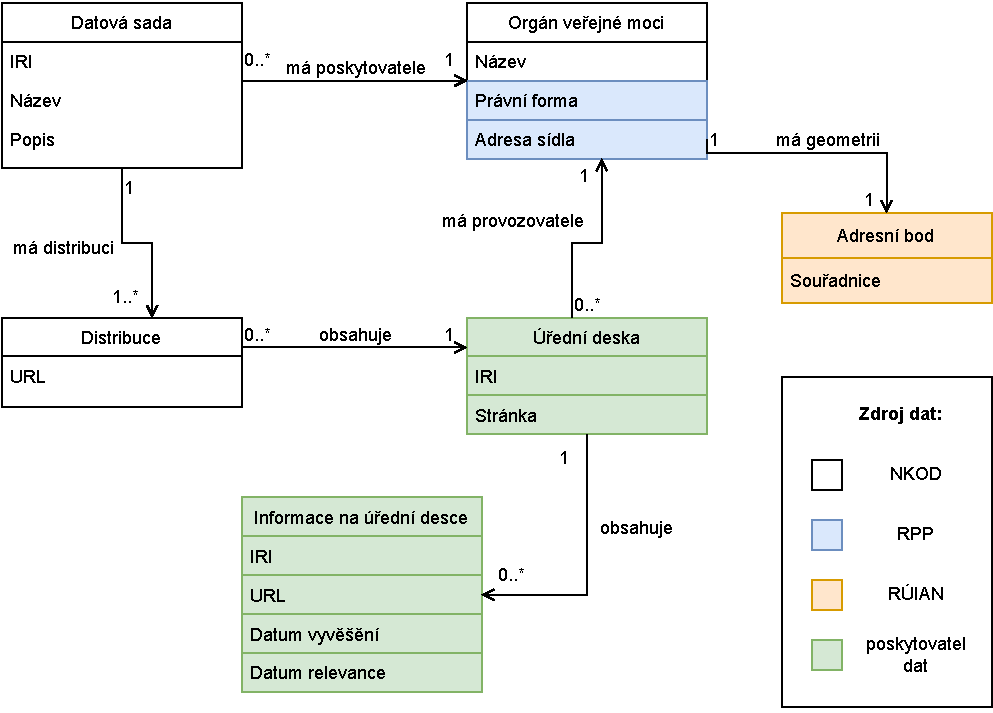
\includegraphics[width=\textwidth]{cs/obrazky/konceptualni_model.pdf}
\caption{Konceptuální model}
\label{fig:konc-model}
\end{figure}

Některé texty v ukázkách dat a některá URL byla pro potřeby práce zkrácena.

\subsection{Datové sady s úředními deskami}

Aplikace používá NKOD k nalezení datových sad s informacemi z úředních desek. Aplikace provádí SPARQL dotazy na endpoint NKOD \footnote{\url{https://data.gov.cz/sparql}}. Následuje příklad SPARQL dotazu (ukázka \ref{code:nkod-dotaz}), který získává z NKOD metadata k datovým sadám s úředními deskami. Dotaz je také možné zobrazit a spustit ve webové aplikaci \href{https://api.triplydb.com/s/aey-LUG7p}{Yasgui}.

%\inputminted{sql}{cs/kod/vsechny_desky.rq}
%\begin{minted}{sql}

\begin{figure}[h]
    \label{code:nkod-dotaz}
    \begin{code}

PREFIX foaf: <http://xmlns.com/foaf/0.1/>
PREFIX dcterms: <http://purl.org/dc/terms/>
PREFIX dcat: <http://www.w3.org/ns/dcat#>
PREFIX l-sgov-sbírka-111-2009-pojem:
<https://slovník.gov.cz/legislativní/sbírka/111/2009/pojem/>

SELECT  ?název ?popis ?poskytovatel ?poskytovatel_iri ?zdroj
WHERE {
    ?s a dcat:Dataset ;
        dcat:distribution ?distribuce ;
        dcterms:conformsTo 
            <https://ofn.gov.cz/úřední-desky/2021-07-20/> ;
        dcterms:title ?název ;
        dcterms:description ?popis;
        dcterms:publisher ?poskytovatel_iri .
    ?distribuce a dcat:Distribution ;
        dcterms:format
            <http://publications.europa.eu/.../file-type/JSON_LD> ;
        dcat:downloadURL ?zdroj .
  FILTER (langMatches(LANG(?název), "cs"))
  FILTER (langMatches(LANG(?popis), "cs"))
  OPTIONAL {
       ?poskytovatel_iri
       l-sgov-sbírka-111-2009-pojem:má-název-orgánu-veřejné-moci
           ?ovm_název_poskytovatele 
  }
  OPTIONAL {
       ?poskytovatel_iri foaf:name ?nkod_název_poskytovatele
  }
  BIND(COALESCE(?ovm_název_poskytovatele, ?nkod_název_poskytovatele)
    AS ?poskytovatel)

}
LIMIT 1
\end{code}
\caption{SPARQL dotaz na NKOD pro získání úředních desek}
\end{figure}

%\end{minted}

Dotaz získá všechny datové sady, které odpovídají specifikaci OFN pro úřední desky \url{https://ofn.gov.cz/úřední-desky/2021-07-20/} pomocí predikátu \\
\texttt{dcterms:conformsTo}. 
V rámci datové sady vybere distribuci ve formátu JSON-LD (predikát \texttt{dcterms:format}) a získá URL distribuce ke stažení (predikát \\ \texttt{dcterms:downloadURL}). 


\begin{figure}[h!]
    \label{code:nkod-res}
\begin{code}
{
  "head": {
    "link": [],
    "vars": [
      "název",
      "popis",
      "poskytovatel",
      "zdroj"
    ]
  },
  "results": {
    "distinct": false,
    "ordered": true,
    "bindings": [
      {
        "název": {
          "type": "literal",
          "xml:lang": "cs",
          "value": "Úřední deska MČ Praha 3"
        },
        "popis": {
          "type": "literal",
          "xml:lang": "cs",
          "value": "Tato datová sada obsahuje data ..."
        },
        "poskytovatel": {
          "type": "literal",
          "xml:lang": "cs",
          "value": "Městská část Praha 3"
        },
        "poskytovatel_iri": {
          "type": "uri",
          "value": 
            "https://rpp-opendata...cz/.../orgán-veřejné-moci/00063517"
        },
        "zdroj": {
          "type": "uri",
          "value": "https://www.praha3.cz/eDeska/opendata"
        }
      }
    ]
  }
}
\end{code}
\caption{Příklad odpovědi z NKOD}
\end{figure}

Z metadat datové sady také získá název (predikát \texttt{dcterms:title}) a popis datové sady (predikát \texttt{dcterms:description}) v českém jazyce a název poskytovatele. U poskytovatele rozlišuje, jestli se jedná o orgán veřejné moci. Pro potřeby práce je výstup omezen 1 výsledek.

Odpověď z NKOD aplikace dostane ve formátu JSON (ukázka \ref{code:nkod-res}). Odpověď obsahuje hlavičku s názvem datový položek, dále následují získaná metadata. Vidíme, že názvy klíčů v ukázce \ref{code:nkod-res} odpovídají názvům proměných ve SPARQL dotazu \ref{code:nkod-dotaz}.

Při zobrazování konkrétní úřední desky, aplikace použije URL distribuce ke stažení dat ze serveru poskytovatele.

IRI datové sady se v aplikaci využívá jako jednoznačný identifikátor úřední desky. Umístěním IRI jako parametru do URL v aplikaci je možné získat odkaz na vizualizaci konkrétní úřední desky. IRI se také používá pro vytvoření odkazu na datovou sadu na webu NKOD.

\subsection{Data z úředních desek}

Samotná data z úředních desek zveřejňuje poskytovatel na adrese, kterou dostaneme jako URL distribuce z dotazu na NKOD popsaného výše. Data pak získáme HTTP požadavkem na dané URL. Data z úředních desek jsou zveřejňovaná ve formátu JSON-LD \cite{JSON-LD} a odpovídají specifikaci OFN pro úřední desky \cite{OFN-UD}.

\begin{figure}[h]
    \label{code:rpp-dotaz}
\begin{code}
PREFIX a-sgov-104-pojem: <https://slovník.gov.cz/agendový/104/pojem/>
PREFIX l-sgov-sbírka-111-2009-pojem:
<https://slovník.gov.cz/legislativní/sbírka/111/2009/pojem/>
PREFIX skos: <http://www.w3.org/2004/02/skos/core#>

SELECT DISTINCT 
    ?nazev ?ico ?cisloPravniFormy ?nazevPravniFormy ?sidlo
WHERE {
  <https://rpp-opendata.egon.gov.cz/.../orgán-veřejné-moci/00063517> 
    a l-sgov-sbírka-111-2009-pojem:orgán-veřejné-moci ;
	l-sgov-sbírka-111-2009-pojem:
	    má-identifikační-číslo-osoby-orgánu-veřejné-moci 
	    ?ico ;
    l-sgov-sbírka-111-2009-pojem:má-právní-formu-osoby 
	    ?pravni_forma ;
  	l-sgov-sbírka-111-2009-pojem:má-název-orgánu-veřejné-moci 
  	    ?nazev ;
    l-sgov-sbírka-111-2009-pojem:má-adresu-sídla-orgánu-veřejné-moci 
        ?sidlo .
  
?pravni_forma   skos:notation ?cisloPravniFormy ;
                skos:prefLabel ?nazevPravniFormy .    
FILTER (LANG(?nazev) = 'cs') 
}
\end{code}
\caption{SPARQL dotaz na RPP - vlastnosti OVM}
\end{figure}

\subsection{Informace o poskytovateli}

V aplikaci je možné třídění úředních desek do kategorií na základě právní formy poskytovatele (obce, kraje, organizační složky státu atp.). 

Jak již bylo popsáno (viz \autoref{subsec:ofn-uredni}) rozlišujeme provozovatele úřední desky a poskytovatele dat v NKOD. Roztřídění úředních desek podle právní formy orgánu aplikace provádí na základě poskytovatele dat z NKOD, tedy ne přímo podle úřadu, který desku spravuje. Toto rozhodnutí můžeme zdůvodnit tím, že ve většině případů se jedná o zaštiťující nebo jinak propojenou organizaci, tedy její právní forma je shodná s právní formou vlastníka desky a je dosaženo stejného výsledku. 

Navíc, získání informace o provozovateli desky je možné pouze z distribuce, tedy pro roztřídění desek do kategorií by bylo nutné stáhnout distribuce všech desek. Toto řešení by se při počtu úředních desek v řádu stovek (a potenciálně tisíců) jevilo jako nevhodné, protože by zbytečně navyšovalo požadavky na připojení uživatele.

Při získávání úředních desek z NKOD v rámci metadat k datové sadě dostaneme název poskytovatele a jeho IRI (viz atributy \texttt{poskytovatel} a \\ \texttt{poskytovatel\_iri} v ukázce dat \ref{code:nkod-res}). IRI se odkazuje do RPP, kde je možné získat další informace o poskytovateli, včetně jeho právní formy a adresy sídla.

Aplikace pro získání těchto dat využívá SPARQL endpoint RPP \footnote{\url{https://rpp-opendata.egon.gov.cz/odrpp/sparql}}. Následuje příklad SPARQL dotazu (ukázka \ref{code:rpp-dotaz}, spustit dotaz v \href{https://api.triplydb.com/s/nPcS7GirV}{Yasgui}) na konkrétní orgán veřejné moci (Městskou část Praha 3) s použitím IRI orgánu, který získá IČO  orgánu (predikát \texttt{má-identifikační-číslo-osoby-orgánu-veřejné-moci}) a jeho právní formu (predikát \texttt{má-právní-formu-osoby}). Z IRI právní formy získá její název a číslo. 

Dotaz také získá adresu sídla orgánu (predikát \\ \texttt{má-adresu-sídla-orgánu-veřejné-moci}), která se využívá pro umístění poskytovatele na mapu.


Odpověď na dotaz z RPP ve formátu JSON je v ukázce \ref{code:rpp-res}. V datech vidíme, že se opravdu jedná o Městskou část Praha 3. Právní forma orgánu je 811, tedy \uv{Městská část, městský obvod}, což odpovídá.
V položce \texttt{sídlo} získáme adresu sídla v podobě IRI adresního místa v RÚIAN.

\begin{figure}
\begin{code}
{
  "head": {
    "link": [],
    "vars": [
      "nazev",
      "ico",
      "cisloPravniFormy",
      "nazevPravniFormy",
      "sidlo"
    ]
  },
  "results": {
    "distinct": false,
    "ordered": true,
    "bindings": [
      {
        "nazev": {
          "type": "literal",
          "xml:lang": "cs",
          "value": "Městská část Praha 3"
        },
        "ico": {
          "type": "typed-literal",
          "datatype": "http://www.w3.org/2001/XMLSchema#string",
          "value": "00063517"
        },
        "cisloPravniFormy": {
          "type": "typed-literal",
          "datatype": "http://www.w3.org/2001/XMLSchema#string",
          "value": "811"
        },
        "nazevPravniFormy": {
          "type": "literal",
          "xml:lang": "cs",
          "value": "Městská část, městský obvod"
        },
        "sidlo": {
          "type": "uri",
          "value": "https://linked.cuzk.cz/.../adresni-misto/21773998"
        }
      }
    ]
  }
}
\end{code}
\caption{Příklad odpovědi z RPP}
\label{code:rpp-res}
\end{figure}

\subsection{Souřadnice adresy sídla}

V aplikaci vizualizujeme úřední desky také na mapě, kam je umístíme podle adresy poskytovatele. Adresu získáme jako IRI adresního místa v RÚIAN. Aby\-chom mohli adresu zobrazit na mapě, potřebujeme z IRI adresního bodu získat souřadnice.

V ukázce \ref{code:ruian-dotaz} můžeme vidět SPARQL dotaz na endpoint RÚI\-AN \footnote{\url{https://linked.cuzk.cz.opendata.cz/sparql}} (spustit dotaz v \href{https://api.triplydb.com/s/7jxqEz6LL}{Yasgui}), který ukazuje, jak získat souřadnice bodu z adresního místa, které získáme jako sídlo orgánu veřejné moci z RPP.

\begin{figure}
    \label{code:ruian-dotaz}
\begin{code}
PREFIX schema: <http://schema.org/>     
PREFIX locn: <http://www.w3.org/ns/locn#>     
SELECT DISTINCT ?geometrie     
WHERE {      
    ?iri    a schema:Place ;          
            locn:geometry ?geometrie .       
VALUES ?iri {
<https://linked.cuzk.cz/resource/ruian/adresni-misto/21773998> 
    } 
}
\end{code}
\caption{SPARQL dotaz na RÚIAN - souřadnice adresního bodu}
\end{figure}


V dotazu používáme klazuli \texttt{VALUES}, do proměnné \texttt{iri} přiřadíme všechna IRI adresních míst, pro která chceme získat souřadnice. V našem příkladu se jedná pouze o jednu adresu (sídlo úřadu městské části Praha 3), v dotazu v aplikaci do klauzule napíšeme IRI adres všech poskytovatelů, u kterých chceme znát souřadnice.

Souřadnice adresního bodu v odpovědi (ukázka \ref{code:ruian-res}) získáme ve formátu Well-Known Text \cite{WKT} --- \texttt{POINT(14.454011740852664 50.08474823342625)}.

\begin{figure}[h]
    \label{code:ruian-res}
\begin{code}
{
  "head": {
    "link": [],
    "vars": [
      "geometrie"
    ]
  },
  "results": {
    "distinct": false,
    "ordered": true,
    "bindings": [
      {
        "geometrie": {
          "type": "typed-literal",
          "datatype": "http://www.opengis.net/ont/gml#wktLiteral",
          "value": "POINT(14.454011740852664 50.08474823342625)"
        }
      }
    ]
  }
}
\end{code}
\caption{Příklad odpovědi z RÚIAN}
\end{figure}
